\documentclass[12pt]{beamer}
%\documentclass[20pt,handout]{beamer}
\usetheme{Darmstadt}
\usepackage{graphicx}
\usepackage[ngerman]{babel}
\usepackage[T1]{fontenc}
\usepackage[utf8]{inputenc}
\usepackage{tikz}
\usepackage[shadow,colorinlistoftodos]{todonotes}
\setbeamertemplate{footline}[frame number]

\newcommand{\cc}[1]{\includegraphics[height=4mm]{img/#1.png}}
\usepackage{ifthen}
\newcommand{\license}[2][]{\\#2\ifthenelse{\equal{#1}{}}{}{\\\scriptsize\url{#1}}}
\usepackage{textcomp}

\setbeamercovered{transparent}

\pgfdeclareimage[height=.6cm]{c3d2logo}{./img/c3d2.pdf} 


\pgfdeclarelayer{foreground}
\pgfsetlayers{main,foreground}
\logo{\pgfputat{\pgfxy(-1,0)}{\pgfbox[center,base]{\pgfuseimage{c3d2logo}}}}


\title{Chaos macht Schule}
\author{\small Robert Wartenberg \& Johannes Lötzsch\\\large Chaos Computer Club Dresden}
\date{16.05.2018}

\begin{document}
\maketitle

\section{Einleitung}
\subsection{}

%%% -> J03 -> %%%

\begin{frame}
  \frametitle{Hacker}
  \begin{figure}
    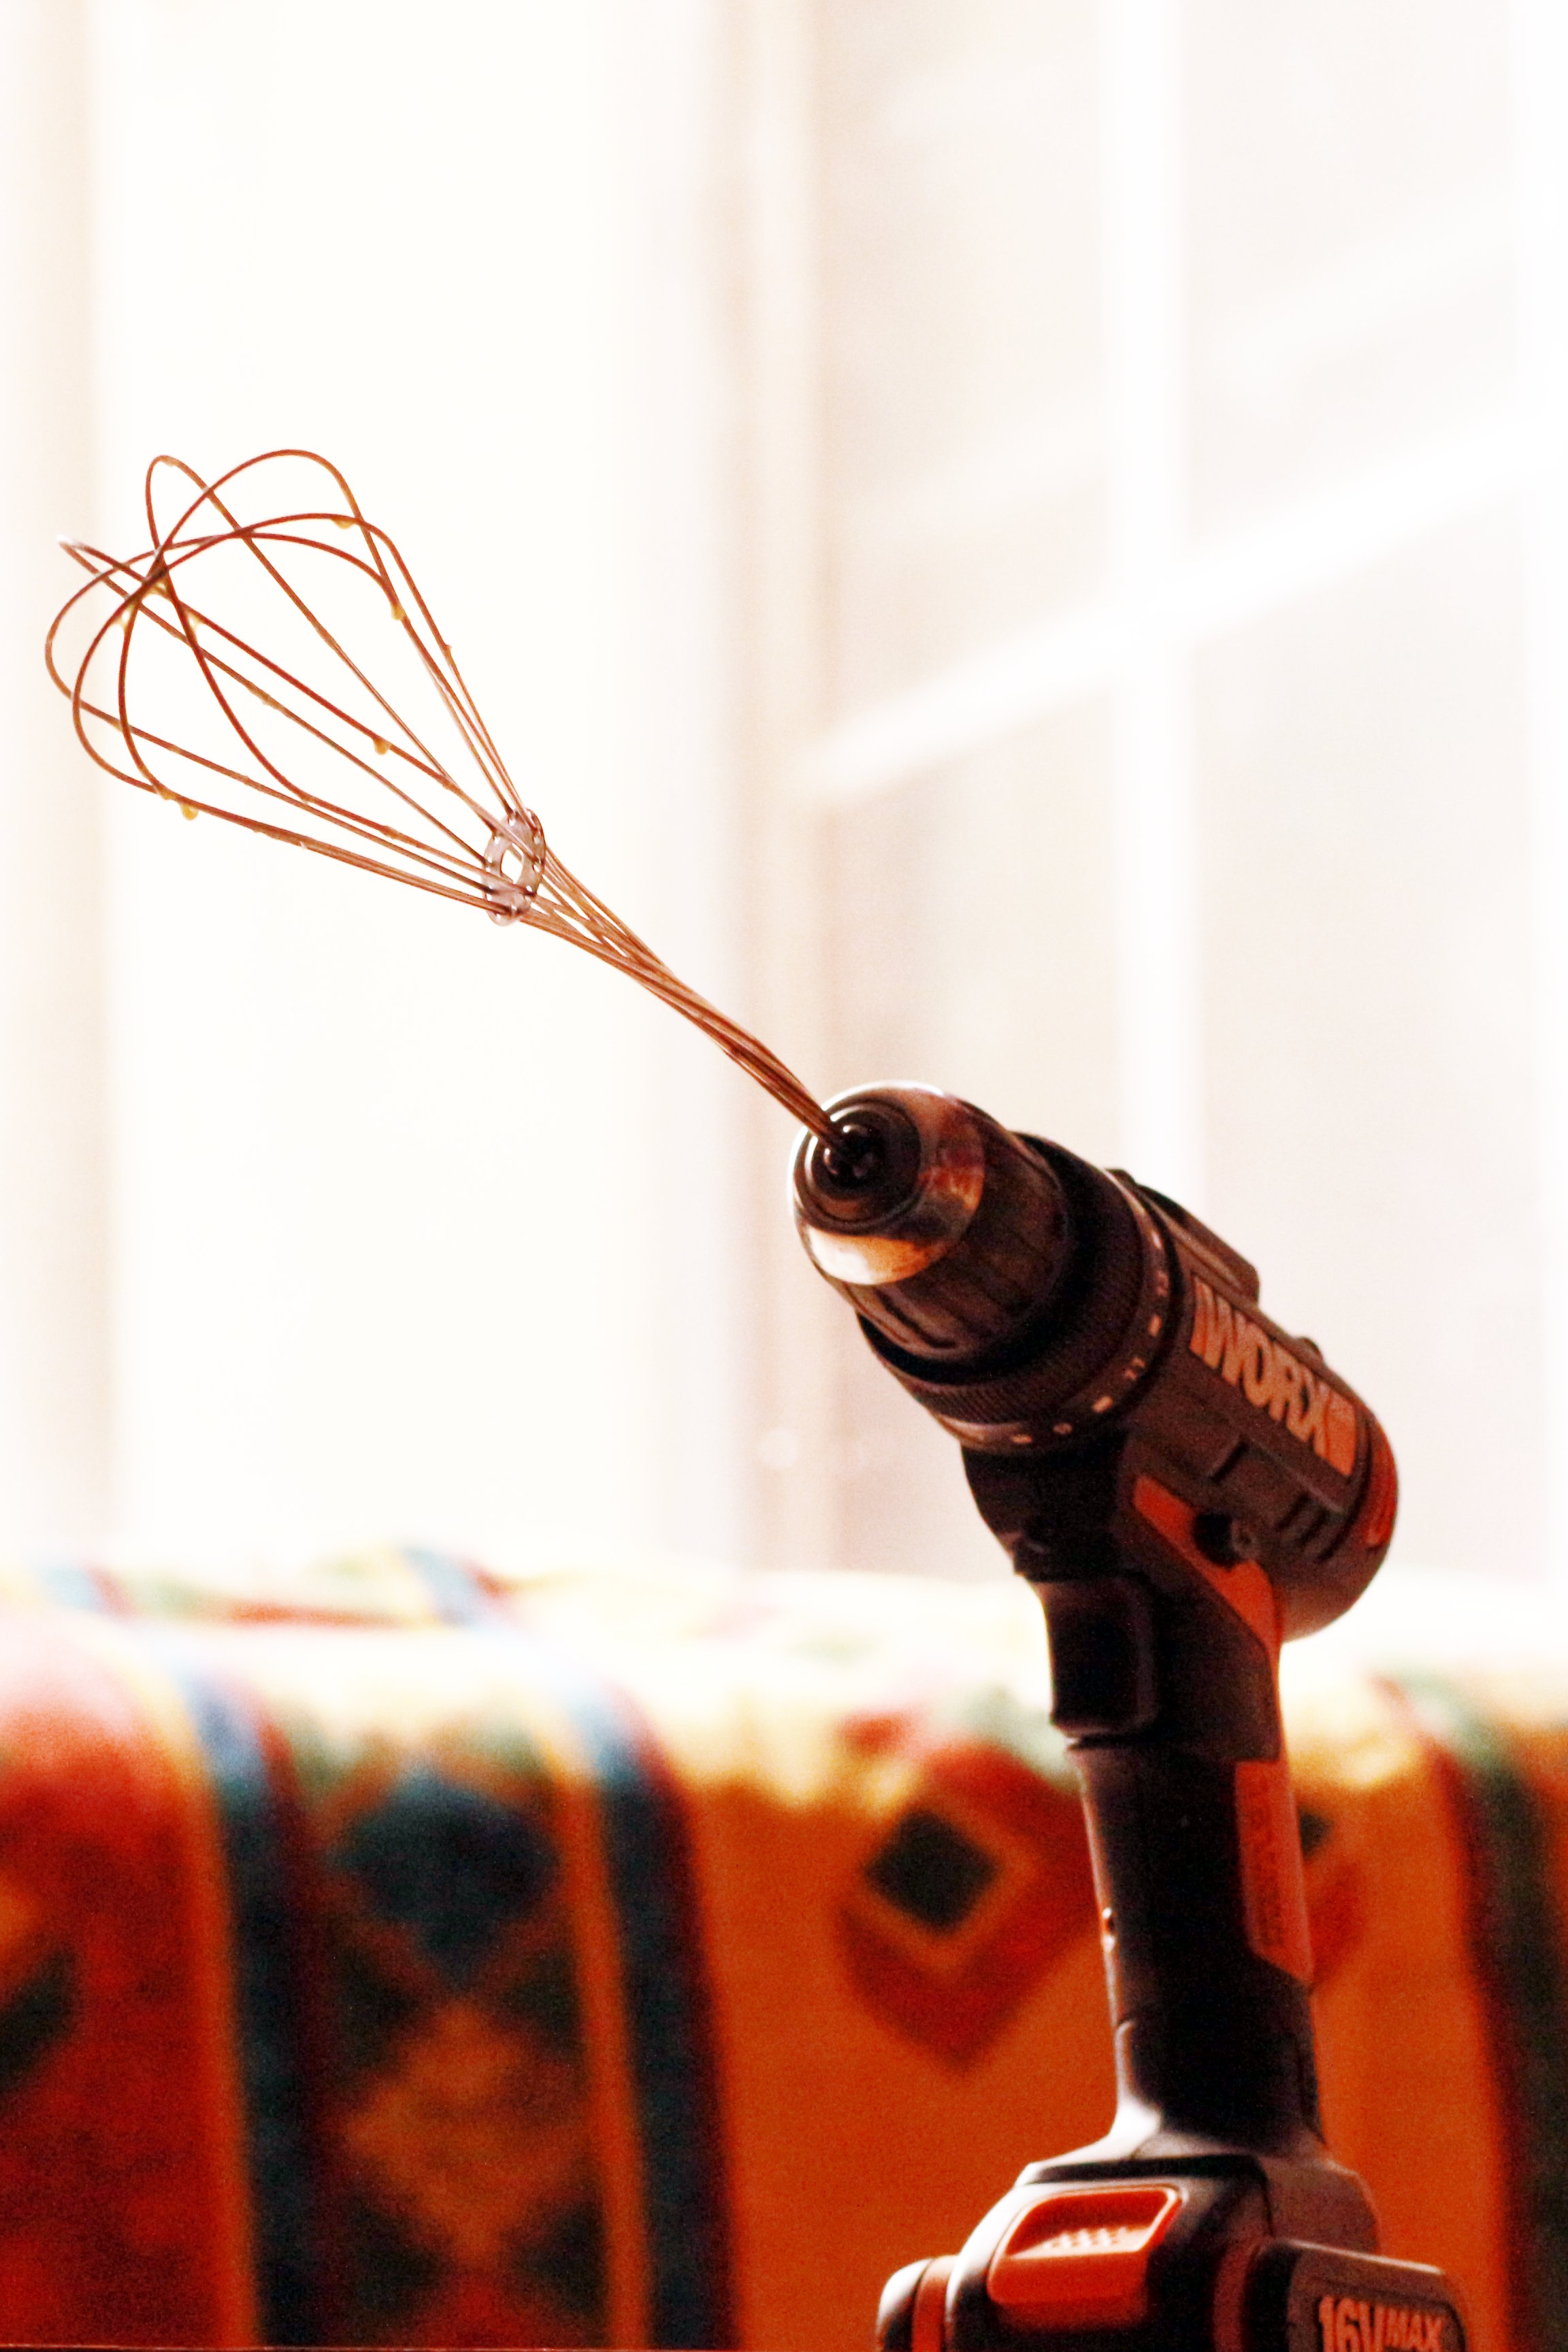
\includegraphics[height=0.7\textheight]{img/schneeschrauber.jpg}
  \end{figure}
\end{frame}

\begin{frame}
	\begin{center}
    	
\includegraphics[height=0.5\textheight]{img/cms-text.png}
    \end{center}
\end{frame}

\begin{frame}
	\frametitle{Chaos Computer Club}
	\begin{center}
		
\includegraphics[height=0.2\textheight]{img/chaosknoten.png}
	\end{center}	
	\begin{itemize}
		\item Verein wurde 1981 gegründet (\url{https://ccc.de})          
		\item Aktuell mehr als 6000 Mitglieder
		\item Betreibt u.a. Öffentlichkeitsarbeit und Politikberatung      
		\item Lokale Erfahrungsaustauschkreise (Erfas) und Chaostreffs
	\end{itemize}
\end{frame}

\begin{frame}
	\frametitle{Chaos Computer Club Dresden}
	\begin{center}
		
\includegraphics[height=0.1\textheight]{img/c3d2_logo.png}
	\end{center}
	\begin{itemize}
		\item Chaos Computer Club Dresden (\url{https://c3d2.de})          
		\item Datenspuren (\url{https://datenspuren.de})
		\item Radio und Podcasts (\url{https://c3d2.de/radio.html})
		\item Chaos macht Schule (\url{https://c3d2.de/schule.html})
	\end{itemize}
\end{frame}
  
%%% -> Rob -> %%%

\section{CmS}
\subsection{}

\begin{frame}
	\begin{center}
    	
\includegraphics[height=0.5\textheight]{img/cms-text.png}
    \end{center}
\end{frame}
  
\begin{frame}
	\frametitle{Chaos macht Schule}
	\begin{itemize}
		\item<1-> seit ca. 2007
		\item<2-> Ehrenamtlich organisiert
		\item<3-> Bildung und Sensibilisierung
	\end{itemize}
\end{frame}
  
\begin{frame}
	\frametitle{Zielgruppe}
	\begin{itemize}
		\item<1-> Schüler*innen
		\item<2-> Lehrer*innen
		\item<3-> Eltern 
	\end{itemize}
\end{frame}
  
%%% -> J03 -> %%%

\begin{frame}
	\frametitle{Inhalte}
	\begin{itemize}
		\item<1-> Datenschutz statt Überwachung
			\only<1>{
				\begin{center}
				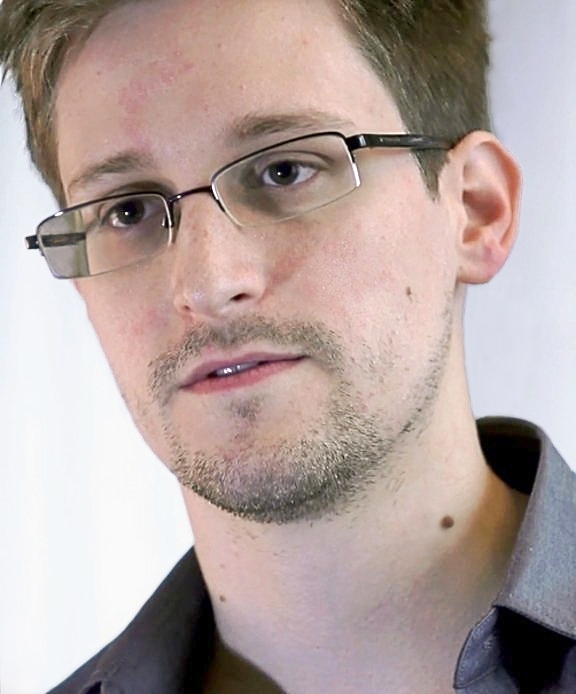
\includegraphics[height=0.7\textheight]{img/snowden.jpg}
				\end{center}
			}
			\only<2>{
				\begin{center}
				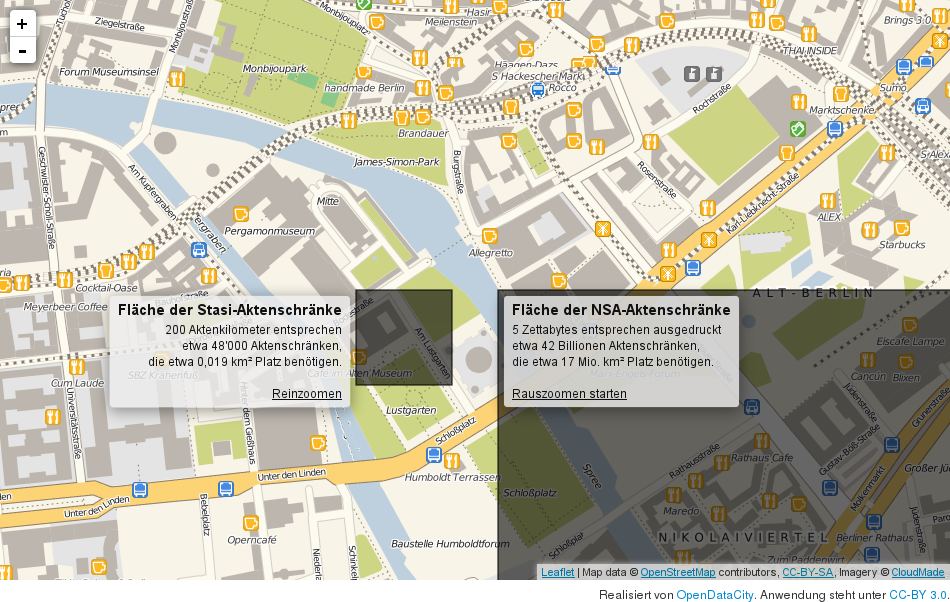
\includegraphics[height=0.7\textheight]{img/akten1.png}
				\end{center}
			}
			\only<3>{
				\begin{center}
				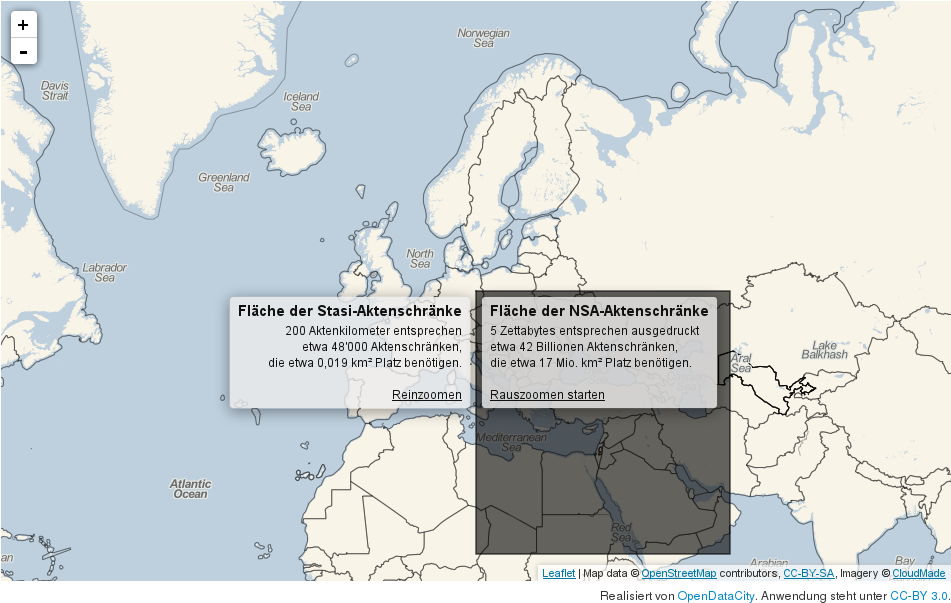
\includegraphics[height=0.7\textheight]{img/akten2.png}
				\end{center}
			}
			\only<4>{
				\begin{center}
				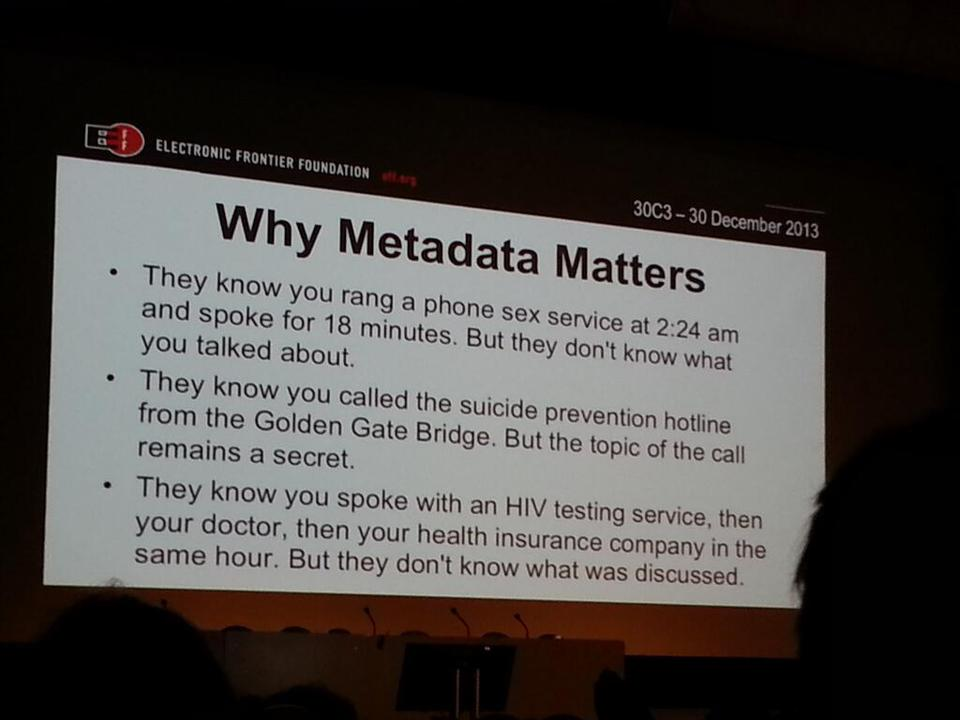
\includegraphics[height=0.7\textheight]{img/metadata-matters.jpg}
				\end{center}
			}
		\item<5-> Sensibilisierung für freie Software \& Dienste
			\only<5>{
				\begin{center}				
				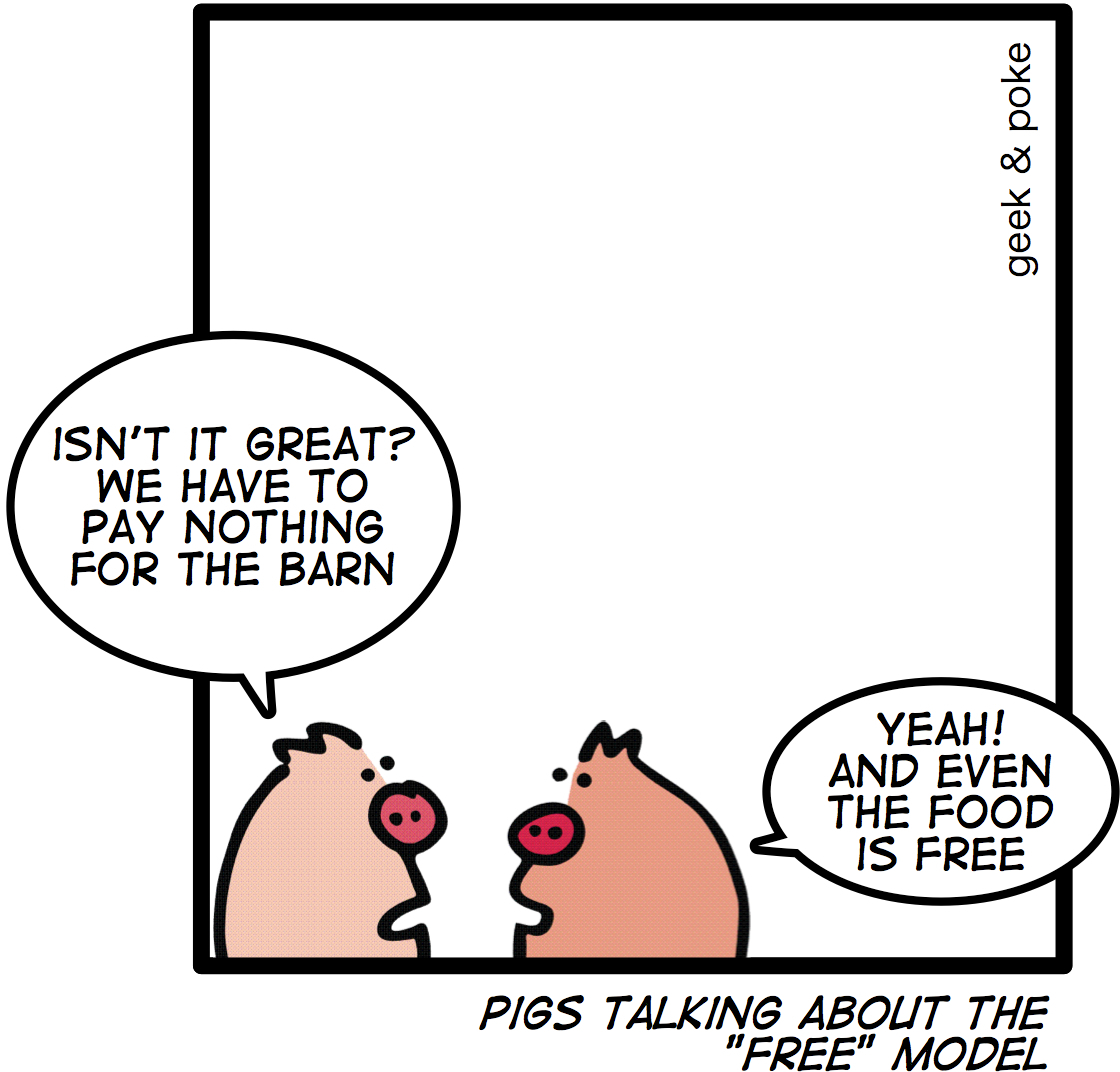
\includegraphics[height=0.7\textheight]{img/business_pigs.jpg}
				\end{center}
			}
		\item<6-> Workshops
			\only<6>{
				\begin{center}
				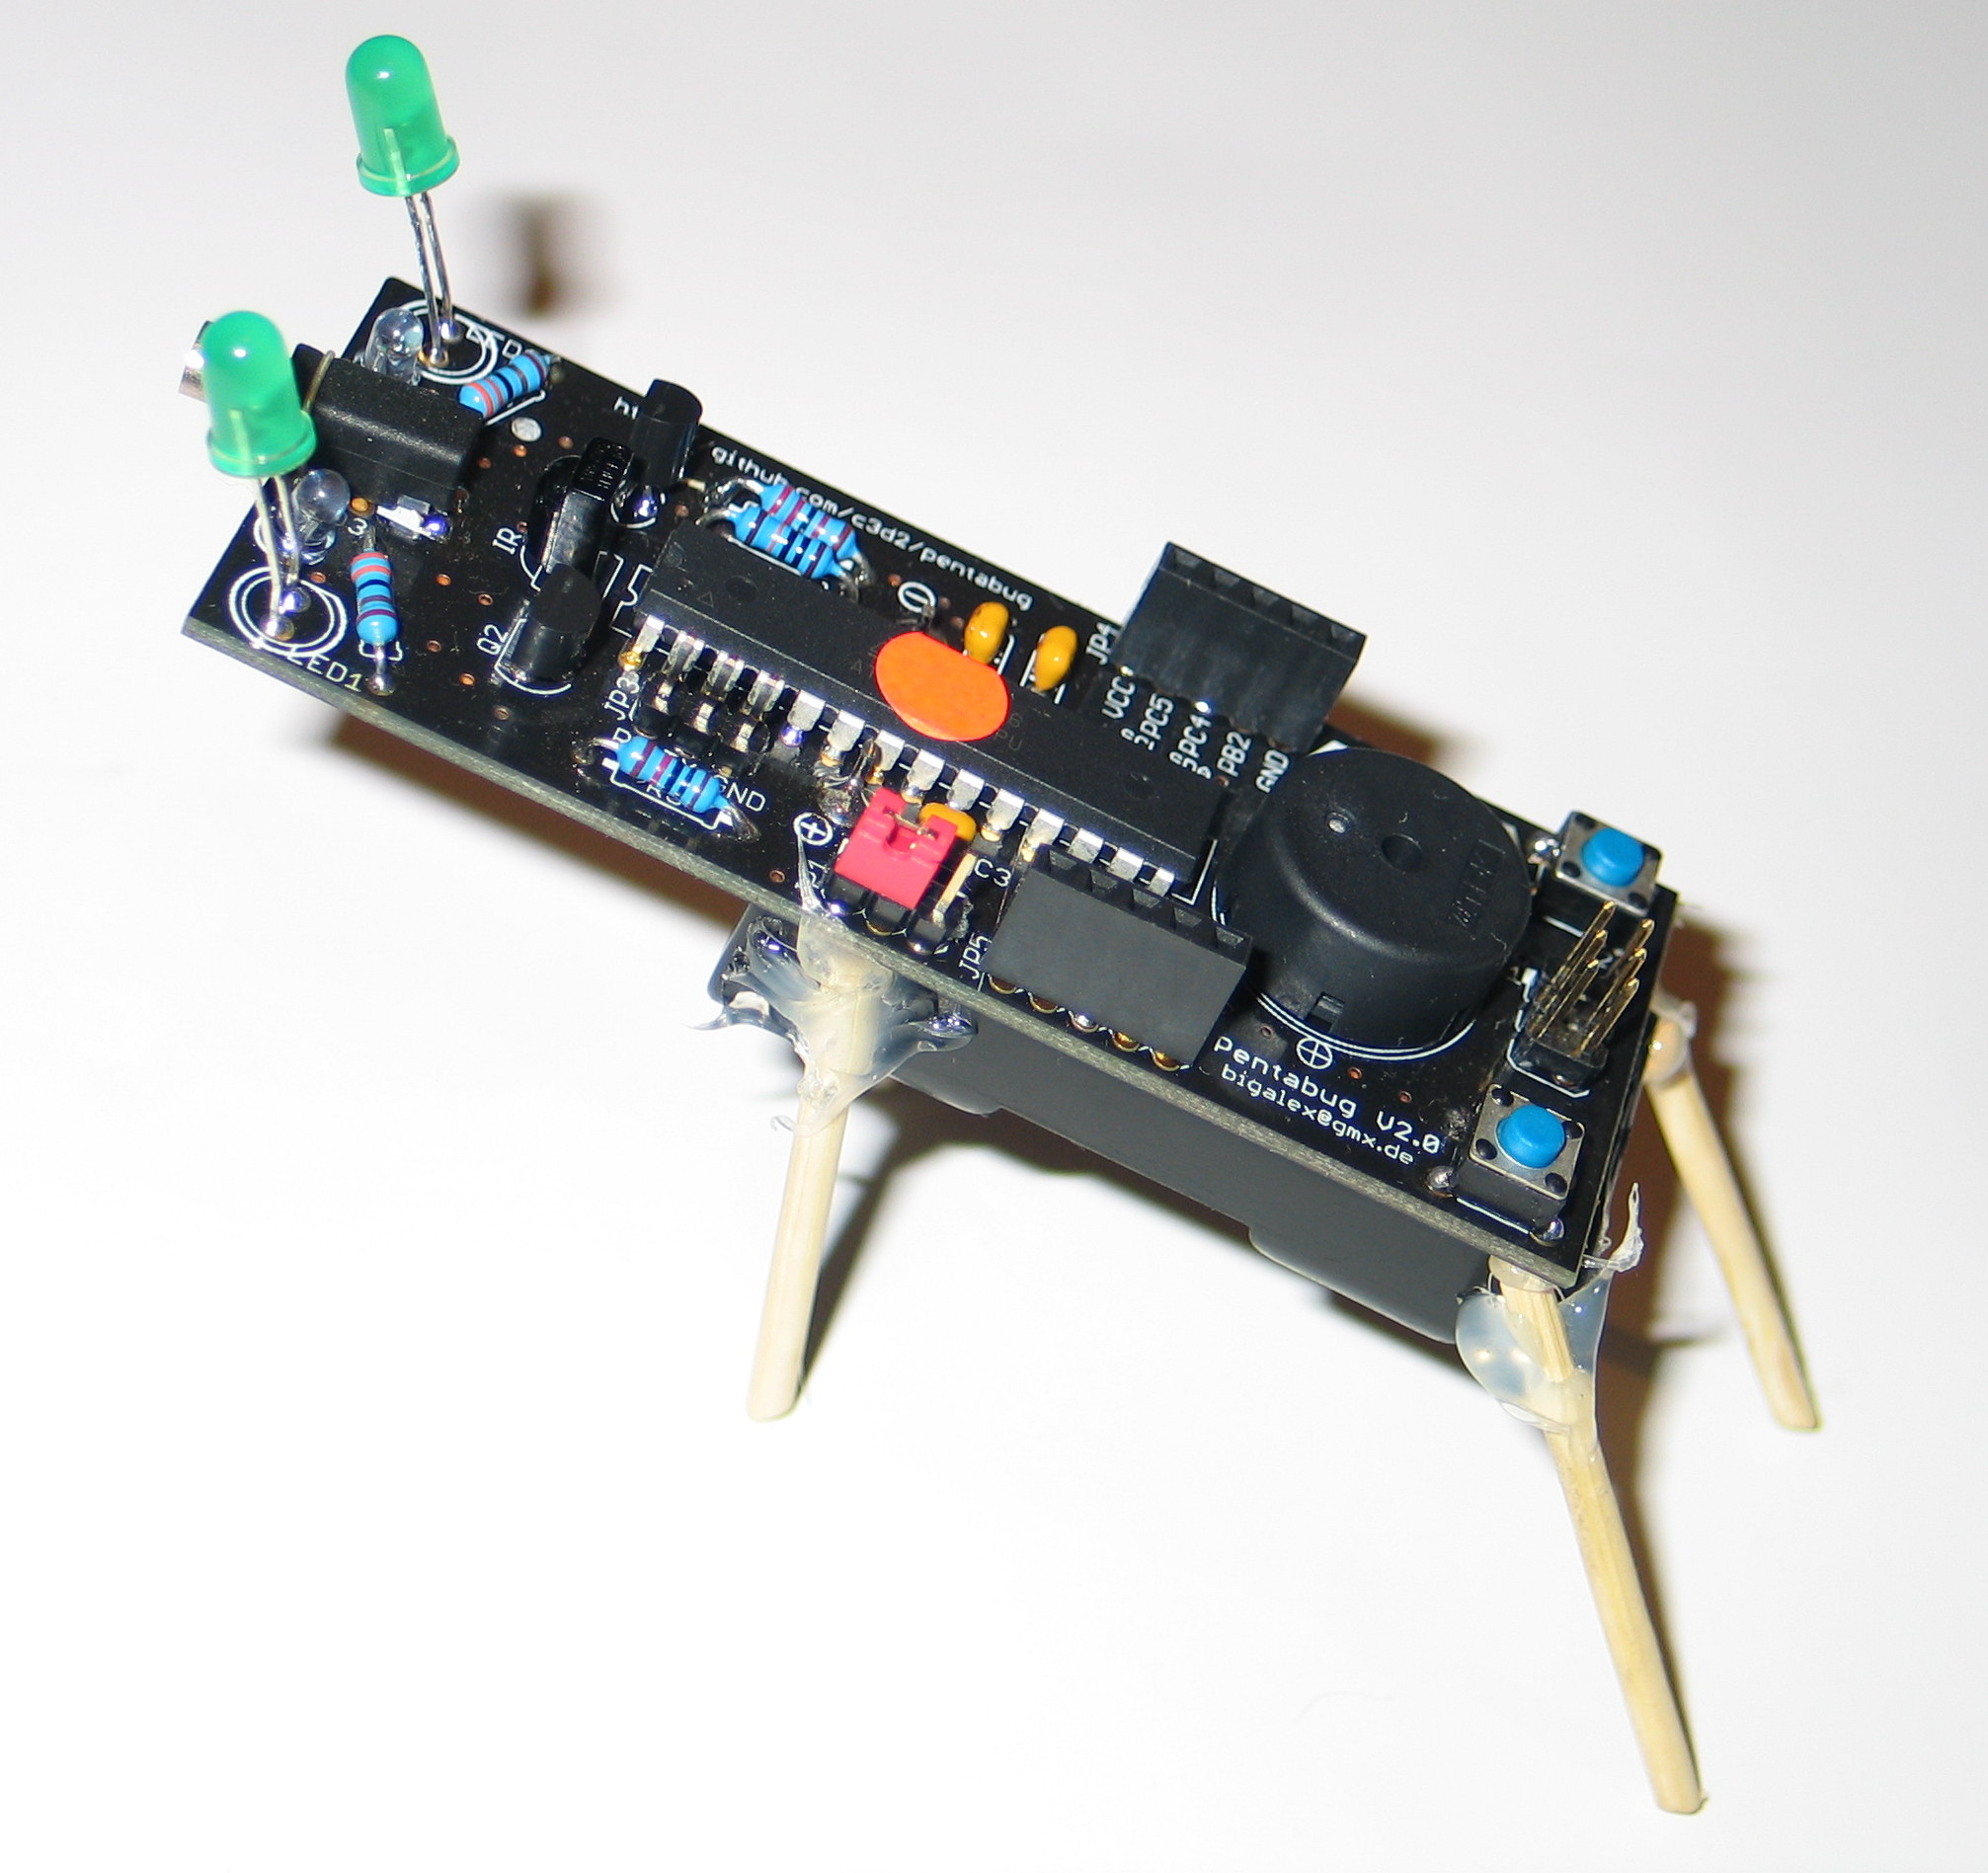
\includegraphics[height=0.5\textheight]{img/pentabug.jpg}
				\end{center}
			}
	\end{itemize}
\end{frame}

%%% -> Rob -> %%%

\section{Internet}
\subsection{}

\begin{center}
\begin{frame}
	\frametitle{Was ist es für ...}
	Kinder?
\end{frame}
\begin{frame}
	\frametitle{Was ist es für ...}
	
\includegraphics[height=0.7\textheight]{img//magic_internet.jpg}
\end{frame}
\begin{frame}
	\frametitle{Was ist es für ...}
	Jugendliche?
\end{frame}
\begin{frame}
	\frametitle{Was ist es für ...}
	
\includegraphics[height=0.7\textheight]{img//social_networks.jpg}
\end{frame}
\begin{frame}
	\frametitle{Was ist es für ...}
	Senioren?
\end{frame}
\begin{frame}
	\frametitle{Was ist es für ...}
	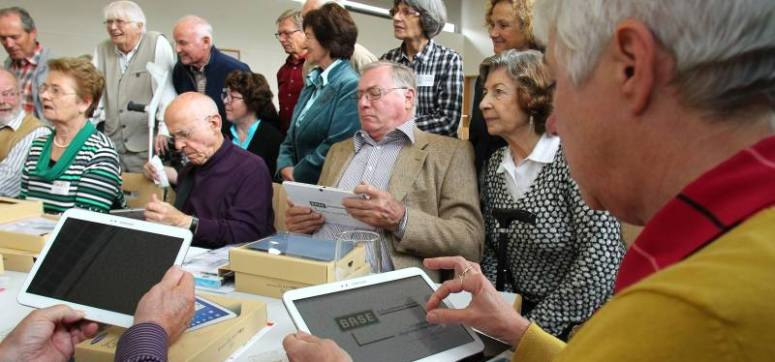
\includegraphics[height=0.5\textheight]{img//senior.jpg}
\end{frame}
\begin{frame}
	\frametitle{Was ist es für ...}
	 euch?
\end{frame}
\begin{frame}
	\frametitle{Was ist es für ...}
	
\includegraphics[height=0.4\textheight]{img//frage.jpg}
\end{frame}
\begin{frame}
	\frametitle{Für uns..}
		\only<1>{
			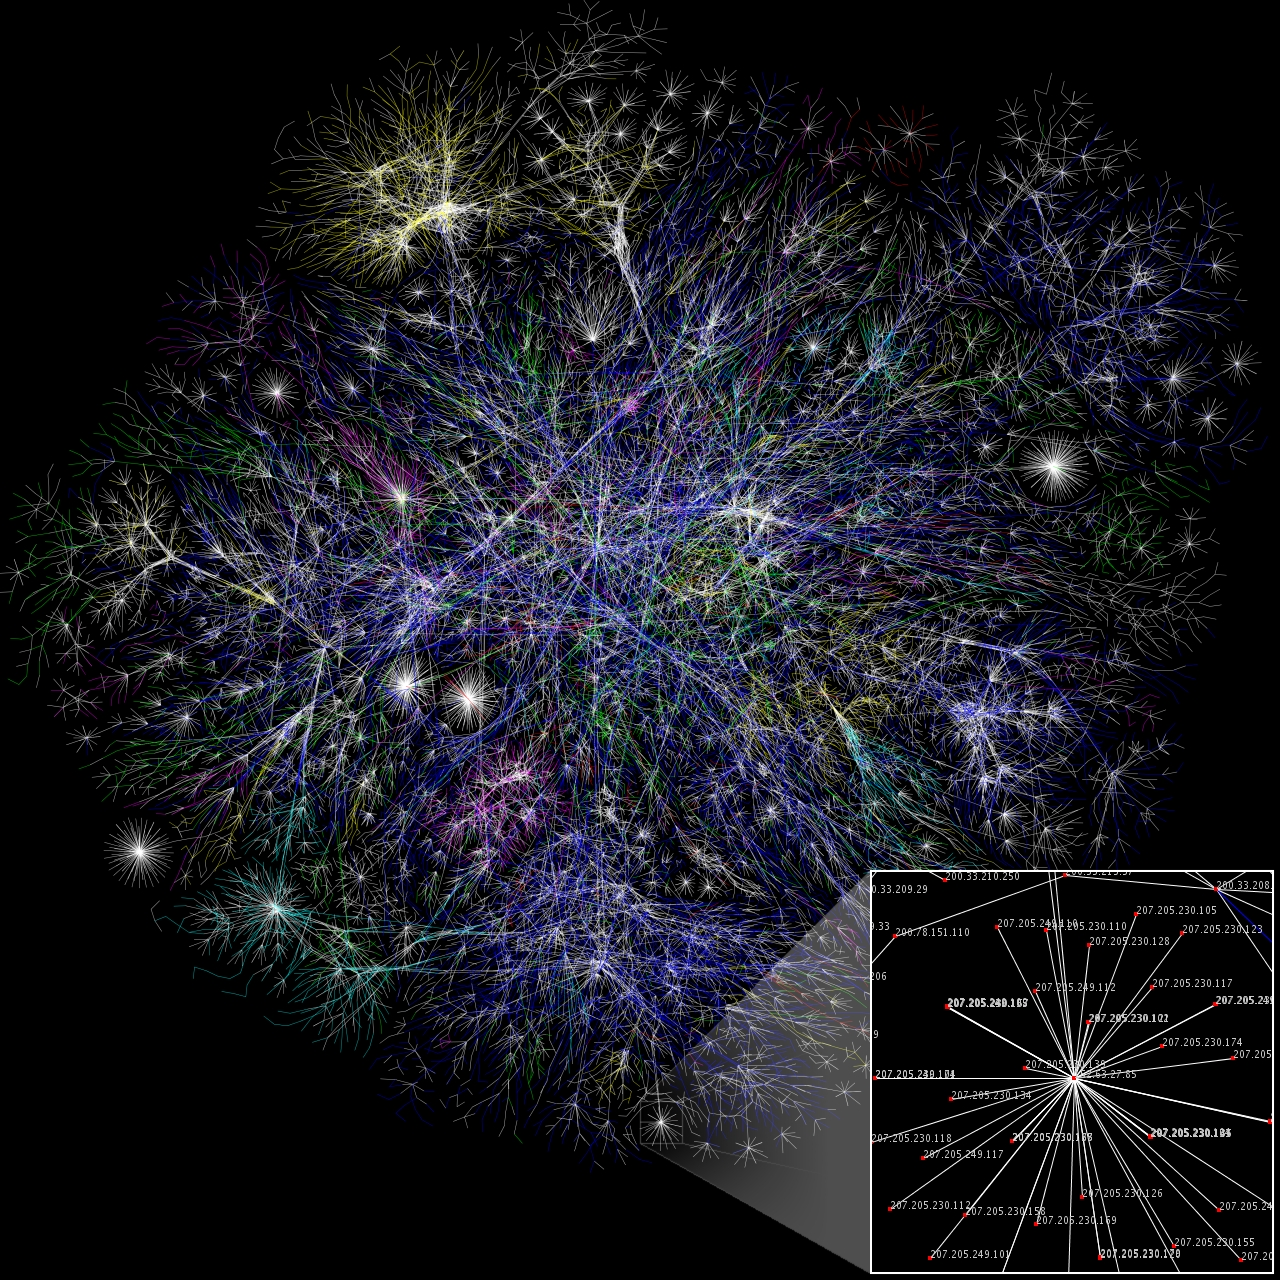
\includegraphics[height=0.7\textheight]{img//internet_0.jpg}
		}
		\only<2>{
			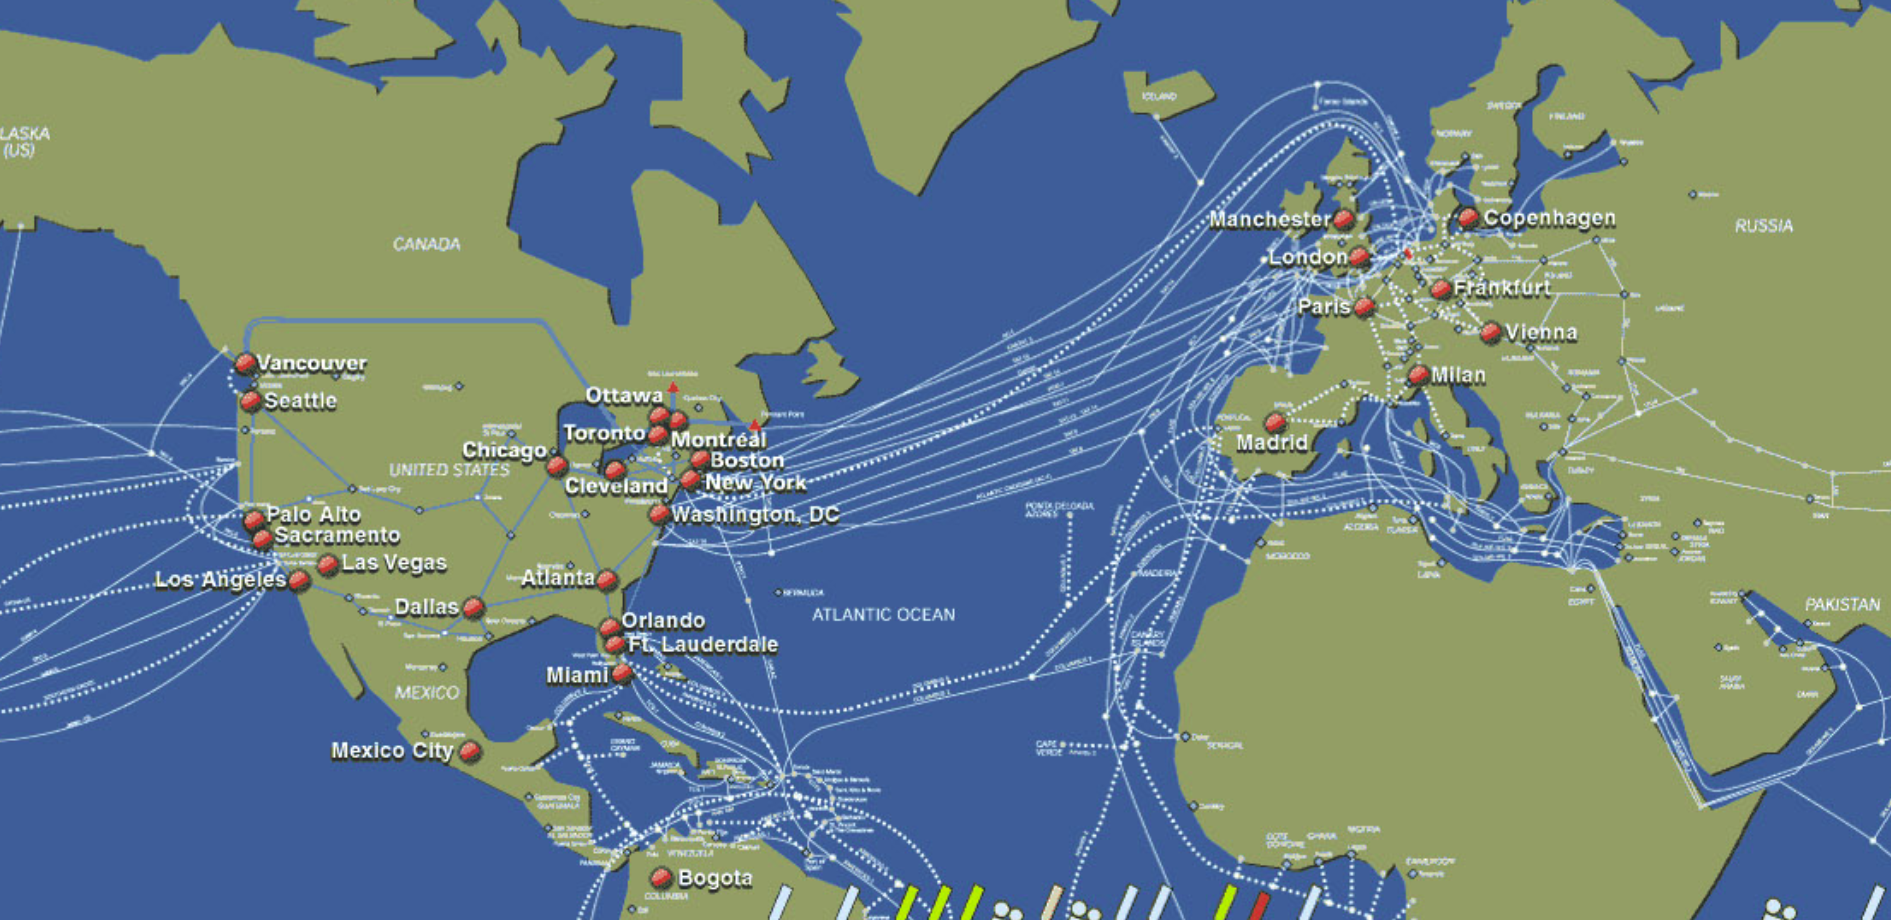
\includegraphics[height=0.6\textheight]{img//internet_1.png}
		}
		\only<3>{
			%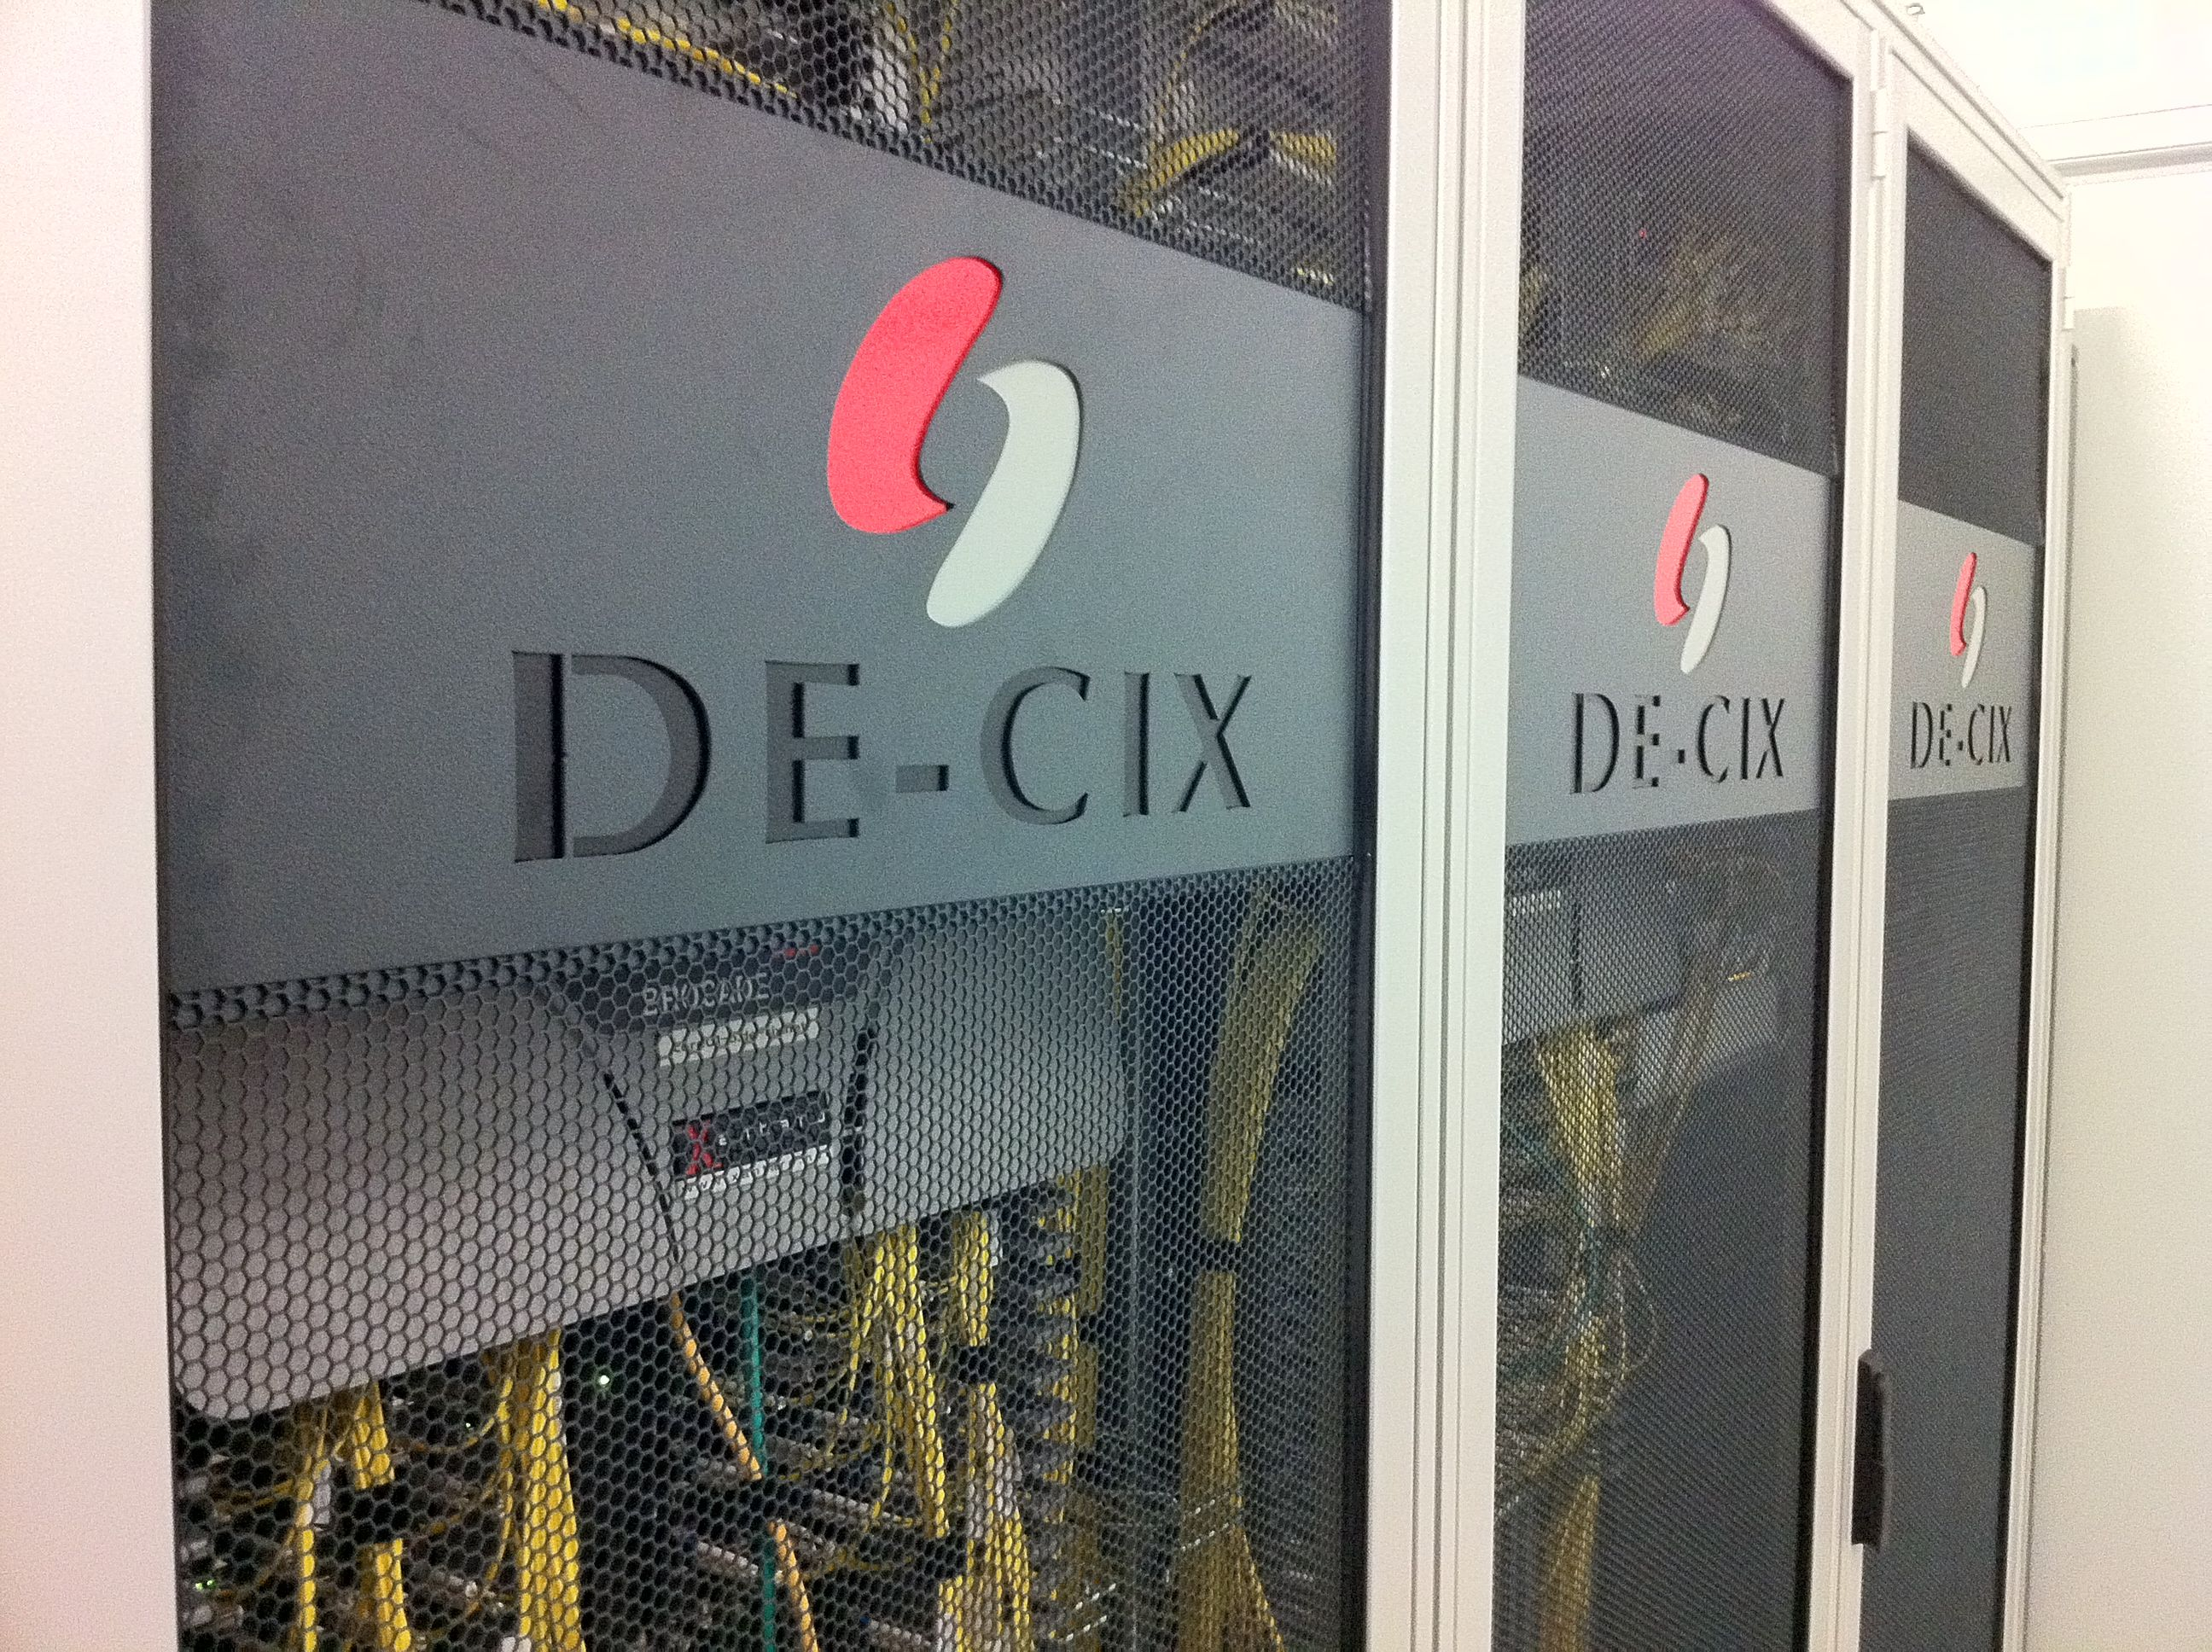
\includegraphics[height=0.6\textheight]{img//internet_2.jpg}
			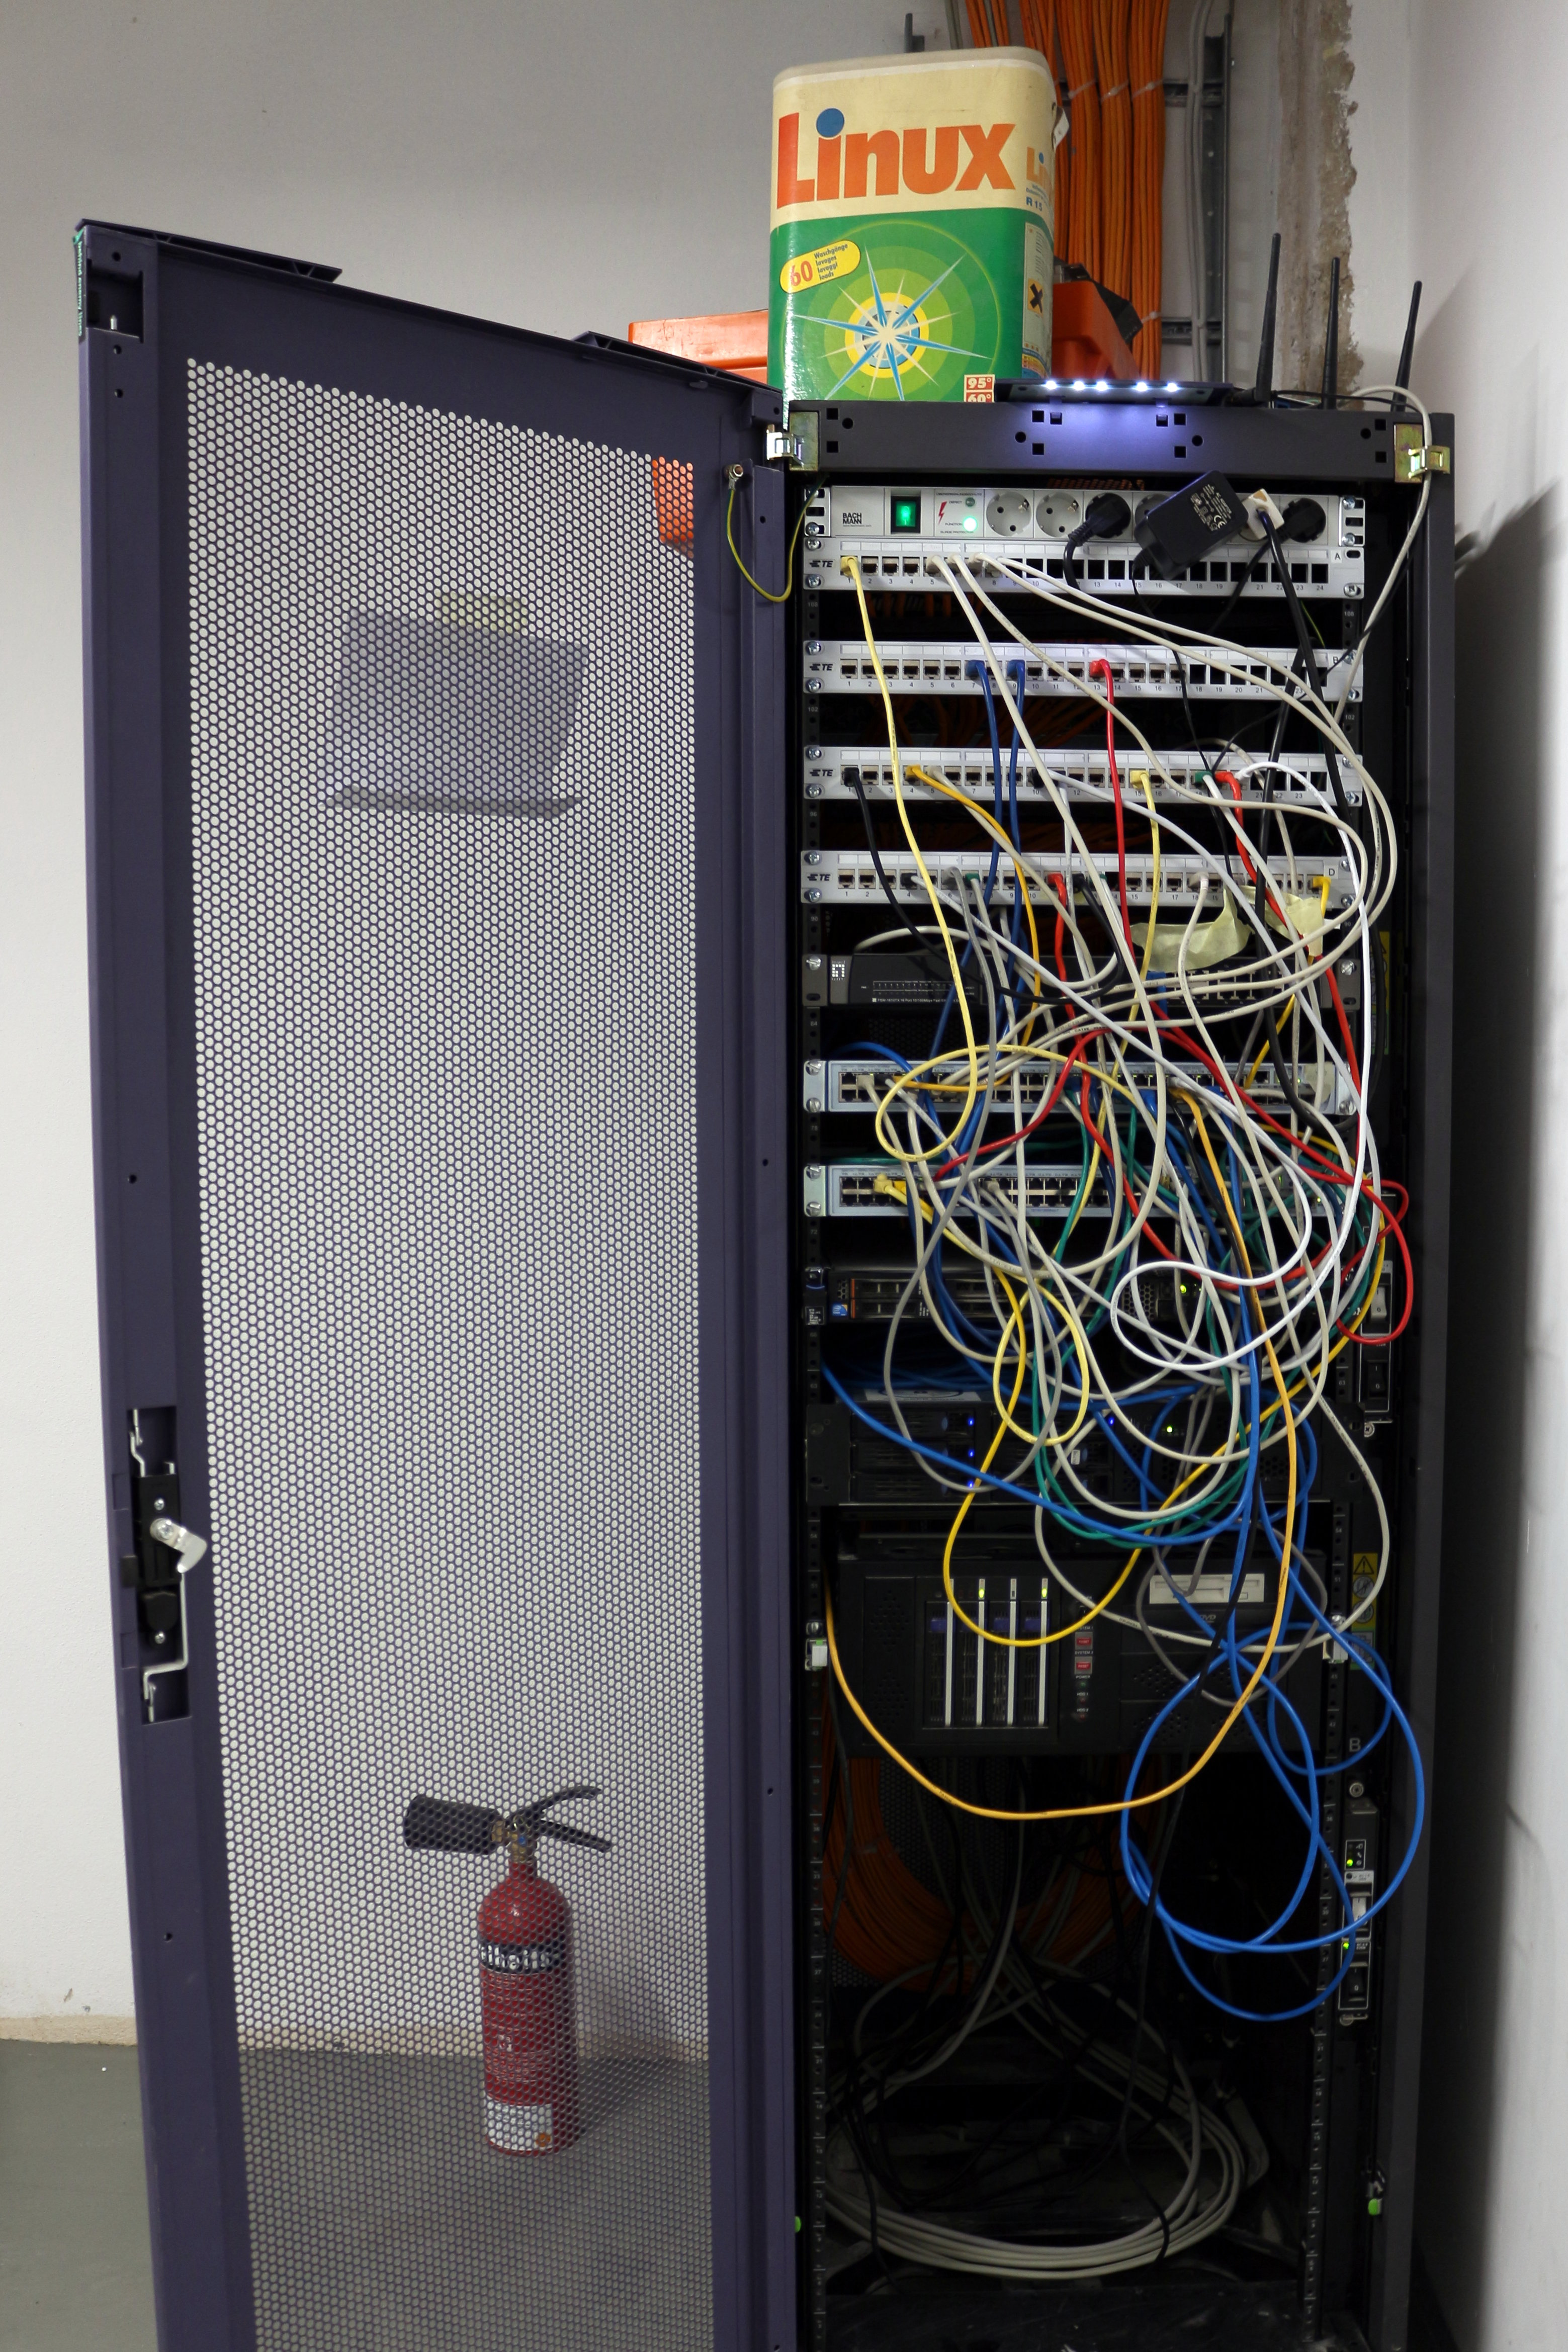
\includegraphics[height=0.6\textheight]{img/rack.jpg}
		}
\end{frame}
\end{center}  

\begin{frame}
	\frametitle{Was macht das Internet groß?}
	\begin{itemize}
		\item<1-> dezentral
		\item<2-> senden und empfangen
    \item<3-> neutral
	\end{itemize}
\end{frame}

\begin{frame}
	\frametitle{Menschen im Internet}
  \begin{itemize}
    \item<1-> Netzwerkeffekte 
    \only<1>{
      \begin{center}
      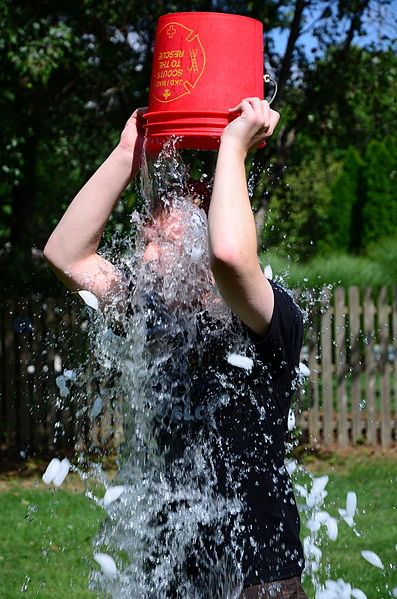
\includegraphics[height=0.5\textheight]{img//Doing_the_ALS_Ice_Bucket_Challenge_wiikipedia.jpg}
      \end{center}
    }
    \item<2-> Echokammern
    \item<3-> digitaler Tribalismus
    \only<3>{
      \begin{minipage}{\linewidth}
          \centering
          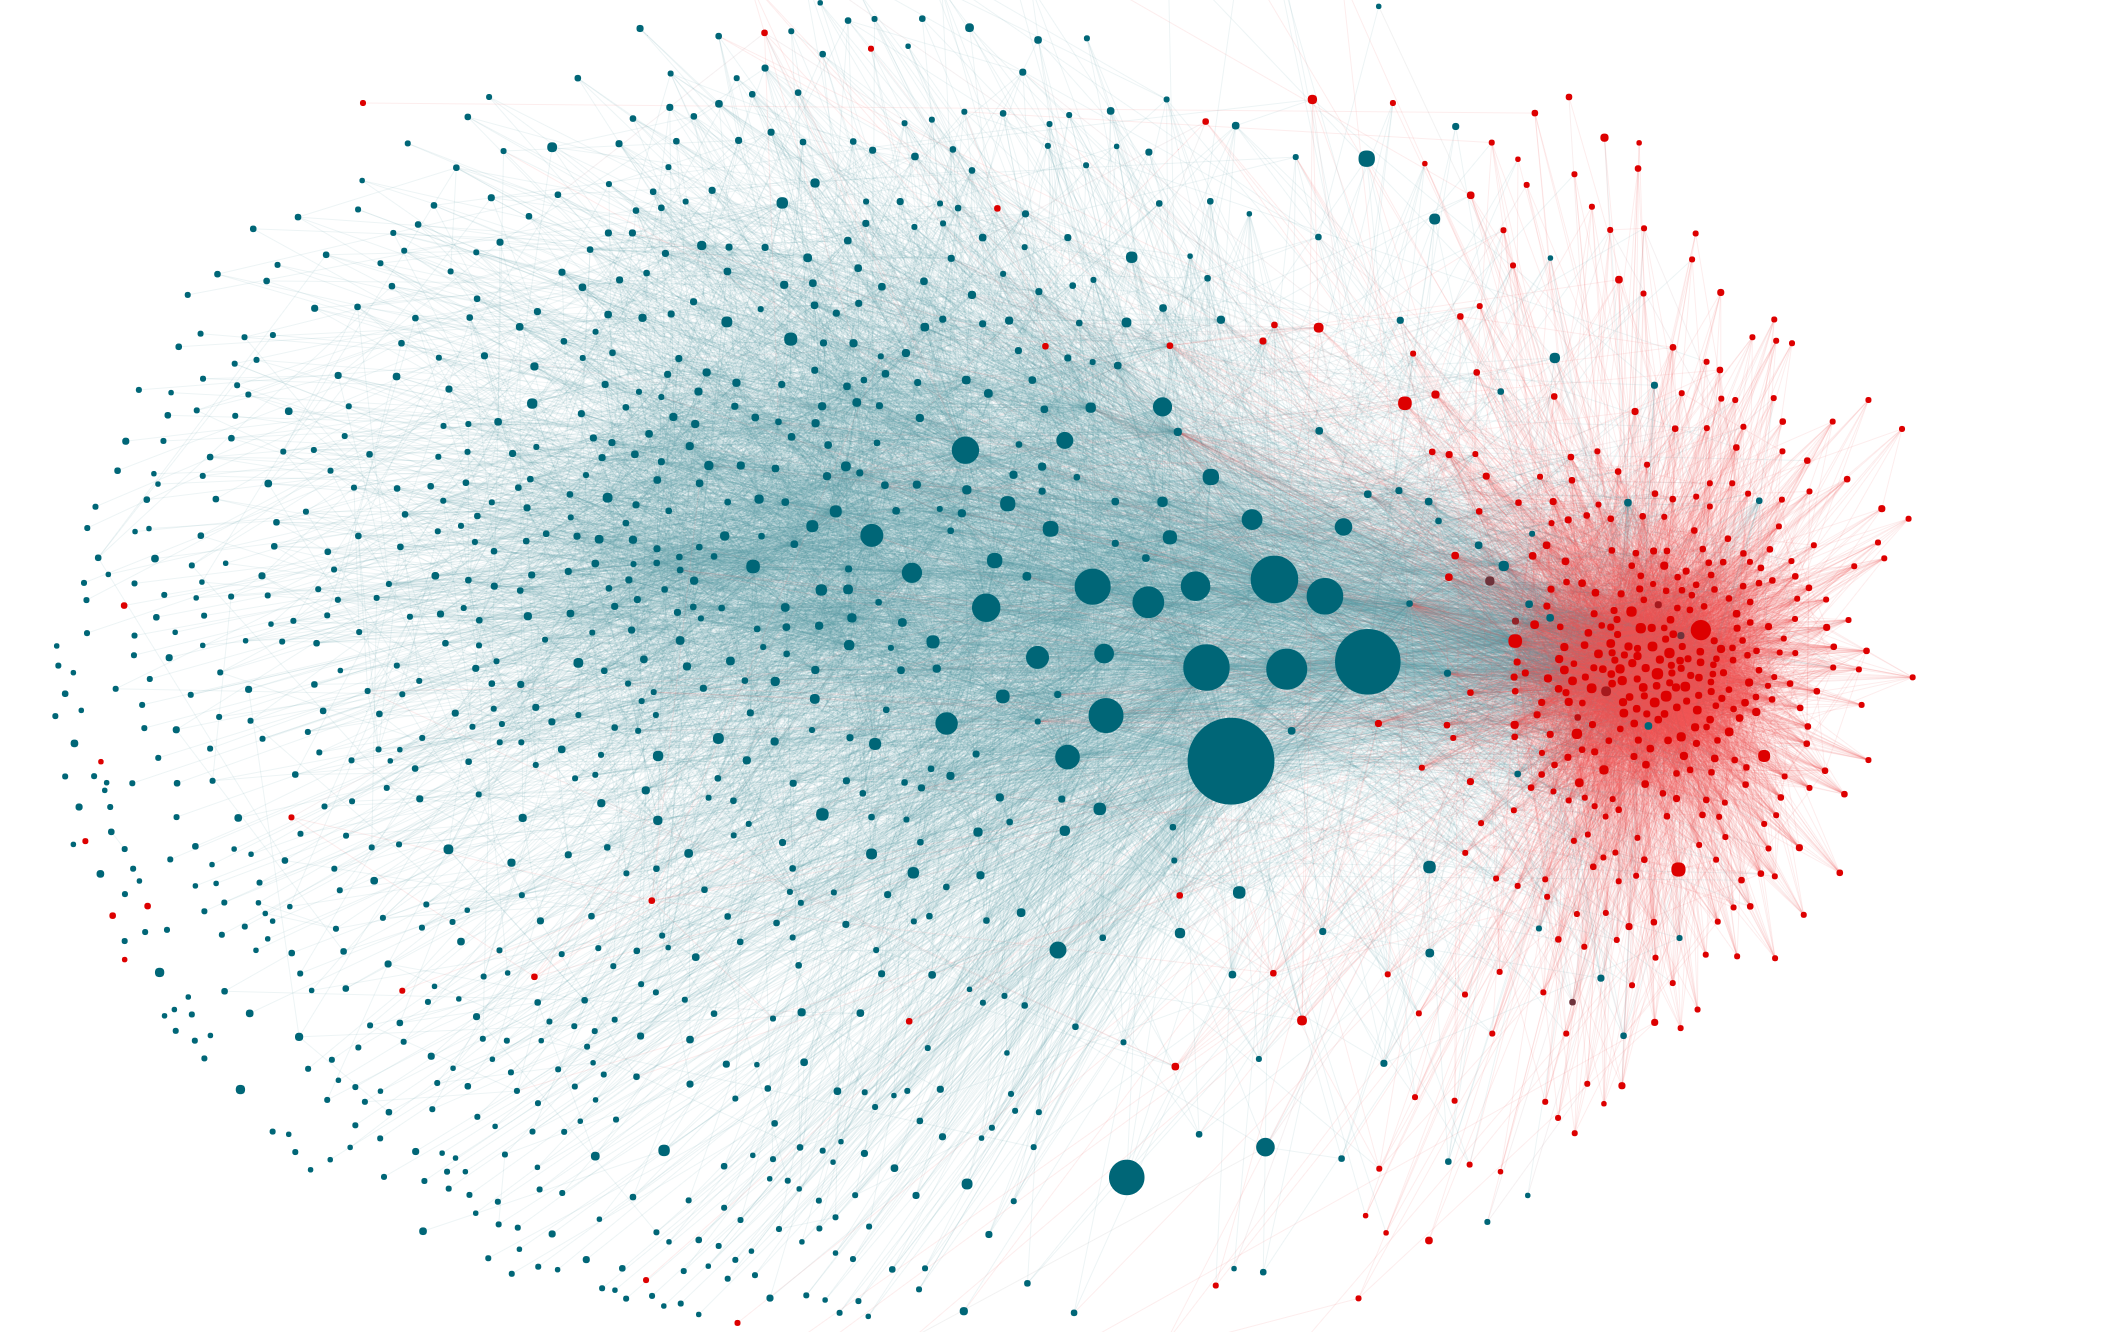
\includegraphics[height=0.5\textheight]{img//digitaler_Tribalismus_Terrorwarnstufe_Schweden.png}
      \end{minipage}
    }      
  \end{itemize}		
\end{frame}

%%% -> J03 -> %%%

\section{Unterricht hacken}
\subsection{}

\begin{frame}
	\frametitle{Display selber bauen}
  	\begin{figure}
	    \only<1>{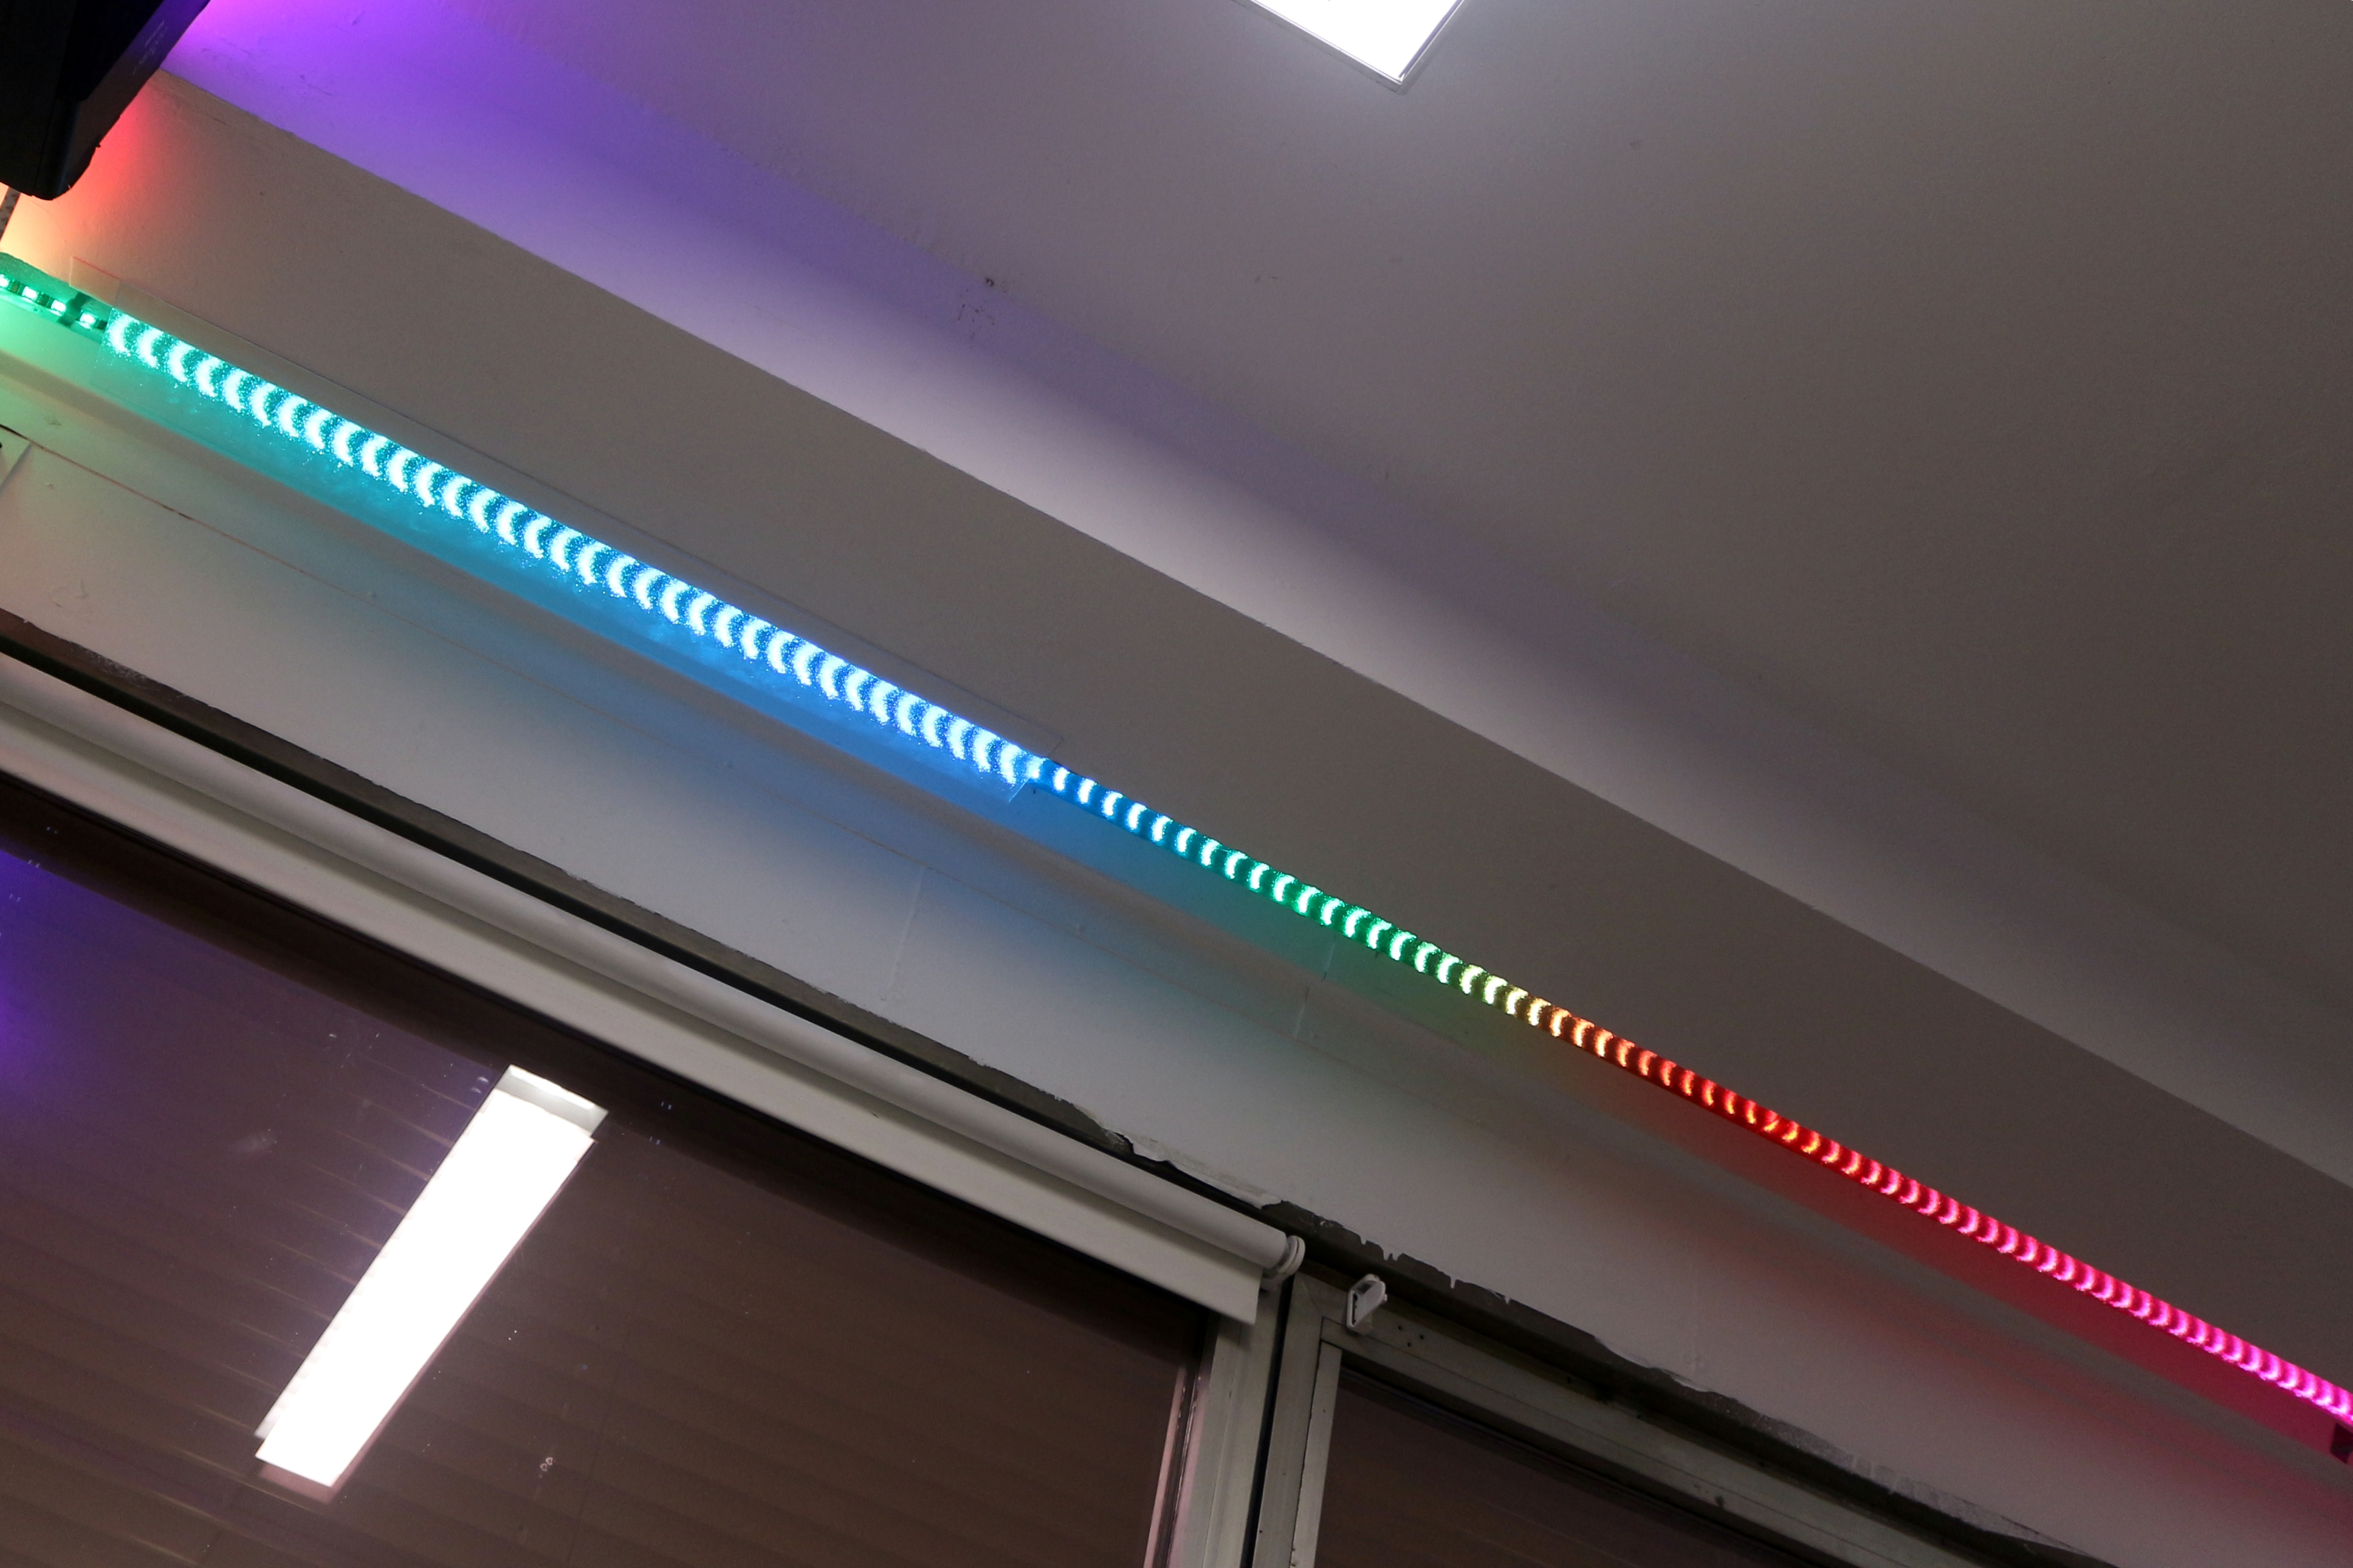
\includegraphics[height=0.7\textheight]{img/leds1.jpg}}
	    \only<2>{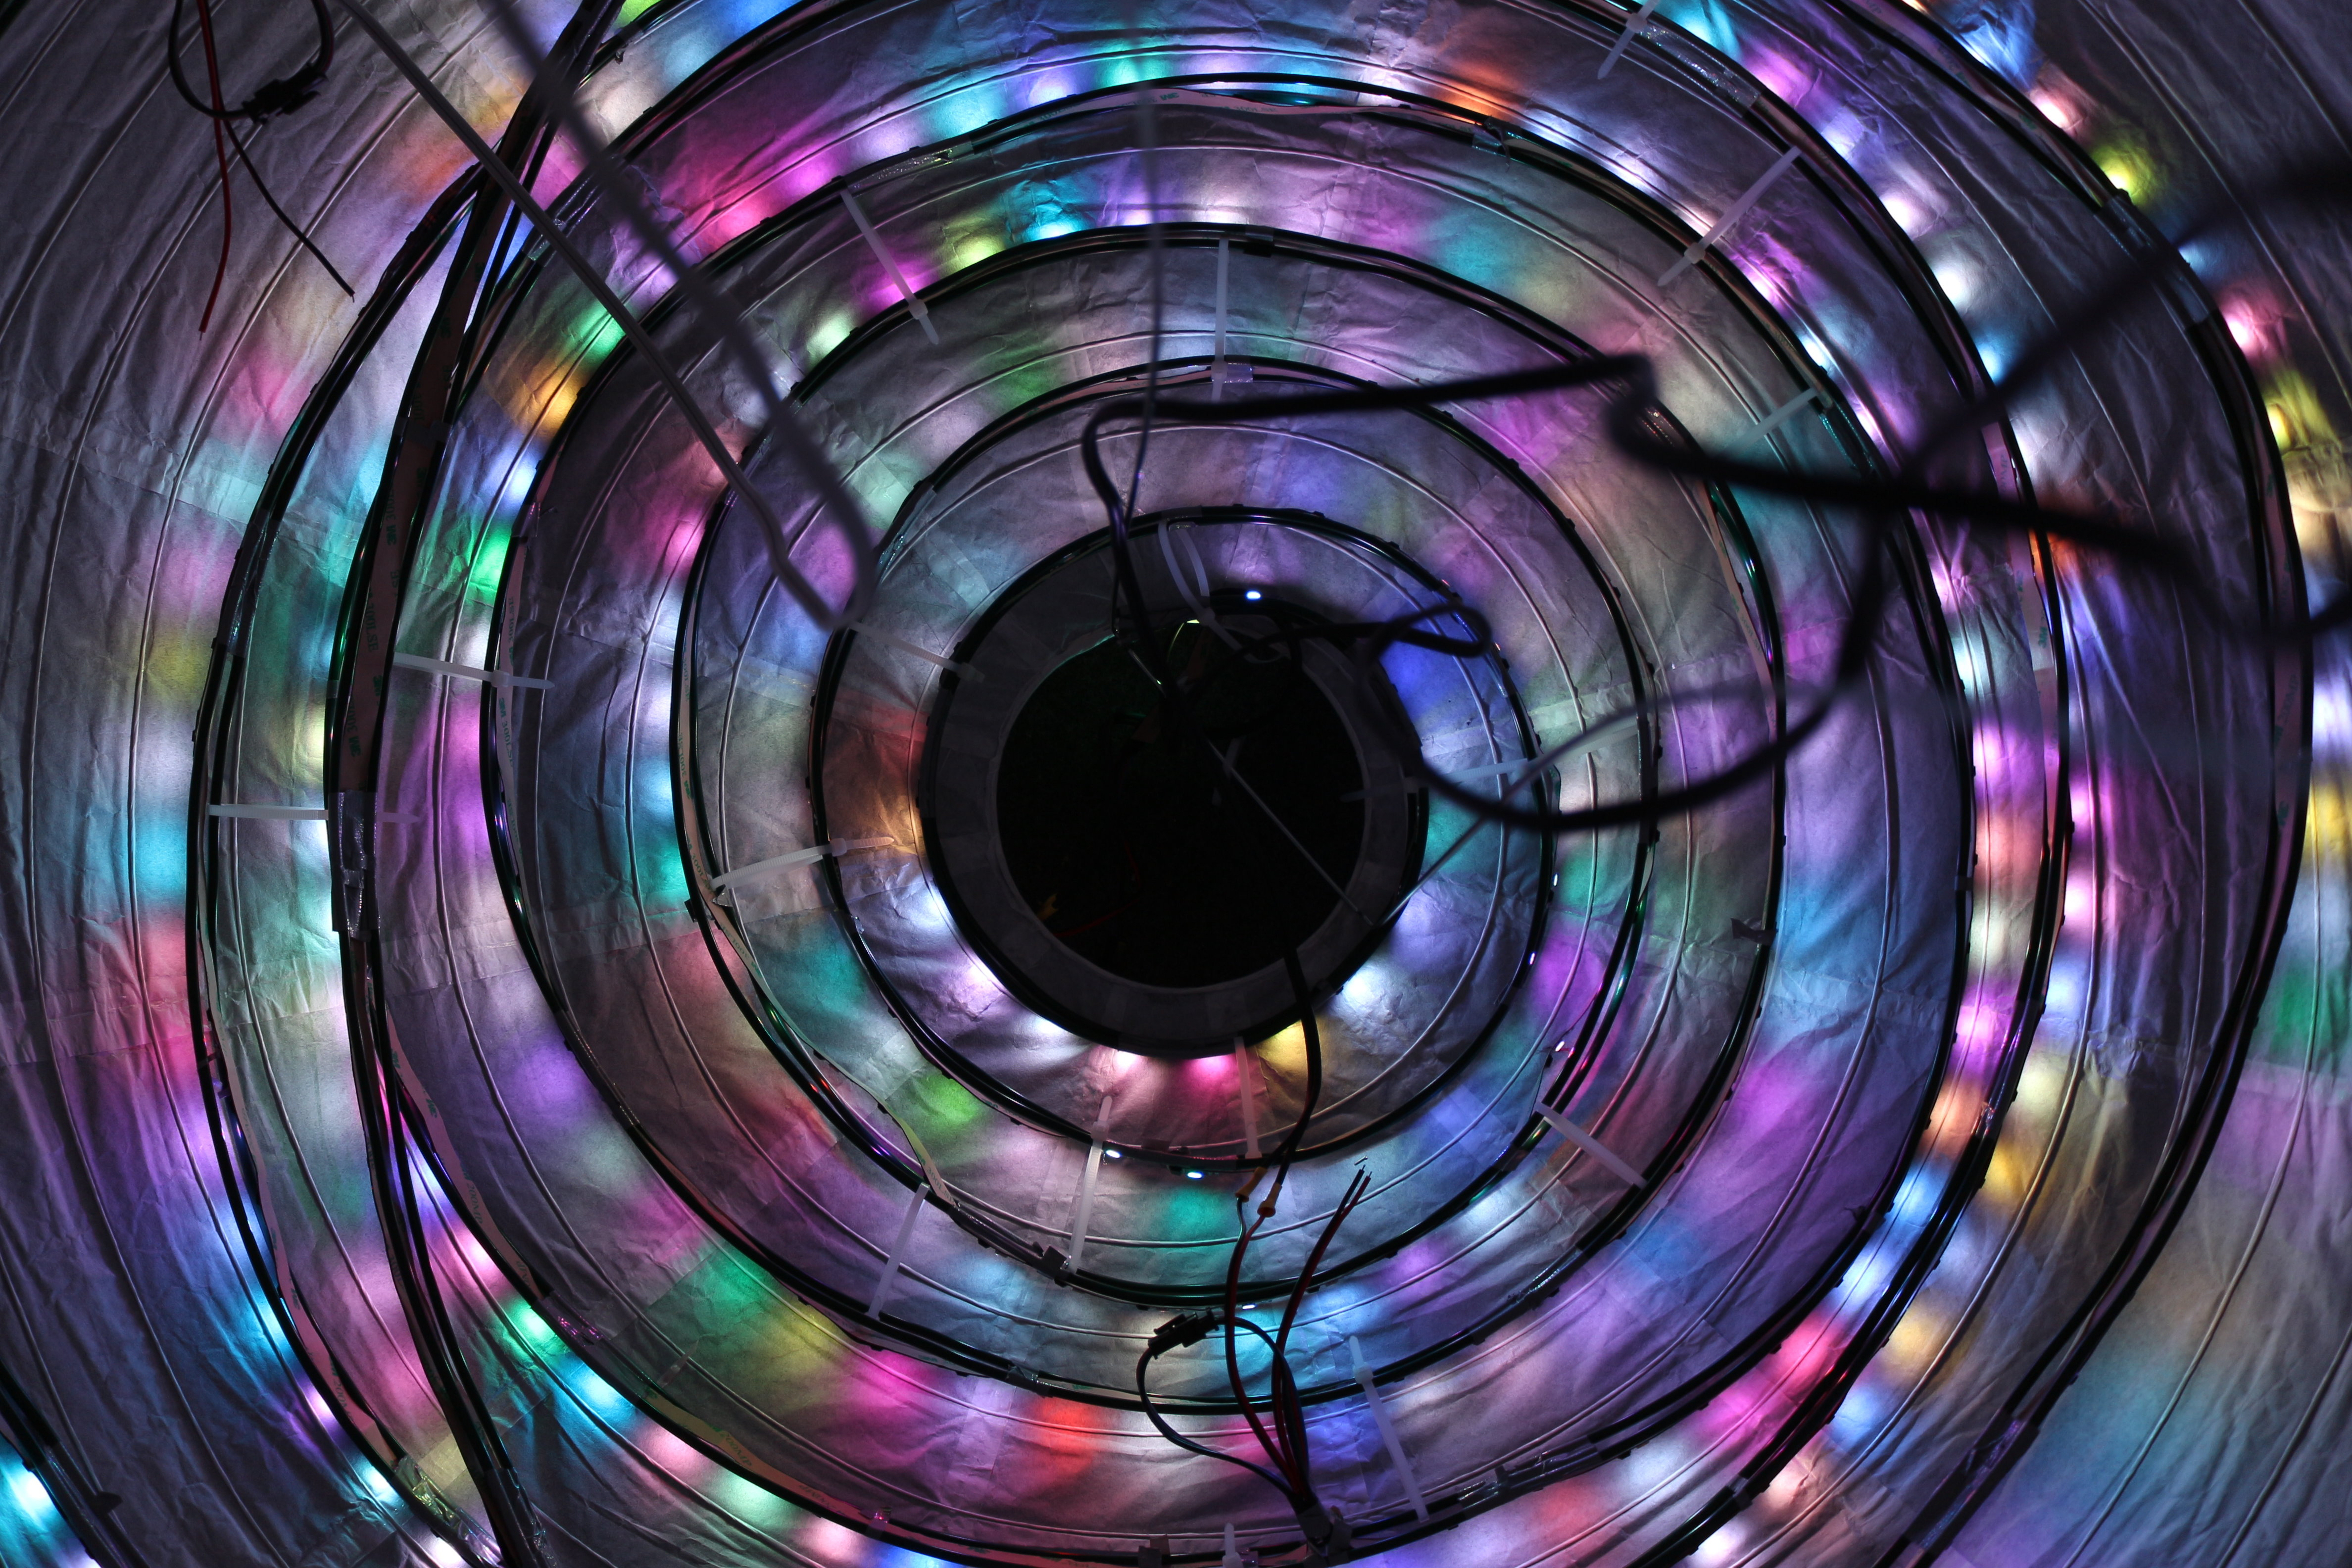
\includegraphics[height=0.7\textheight]{img/leds2.jpg}}
	    \only<3>{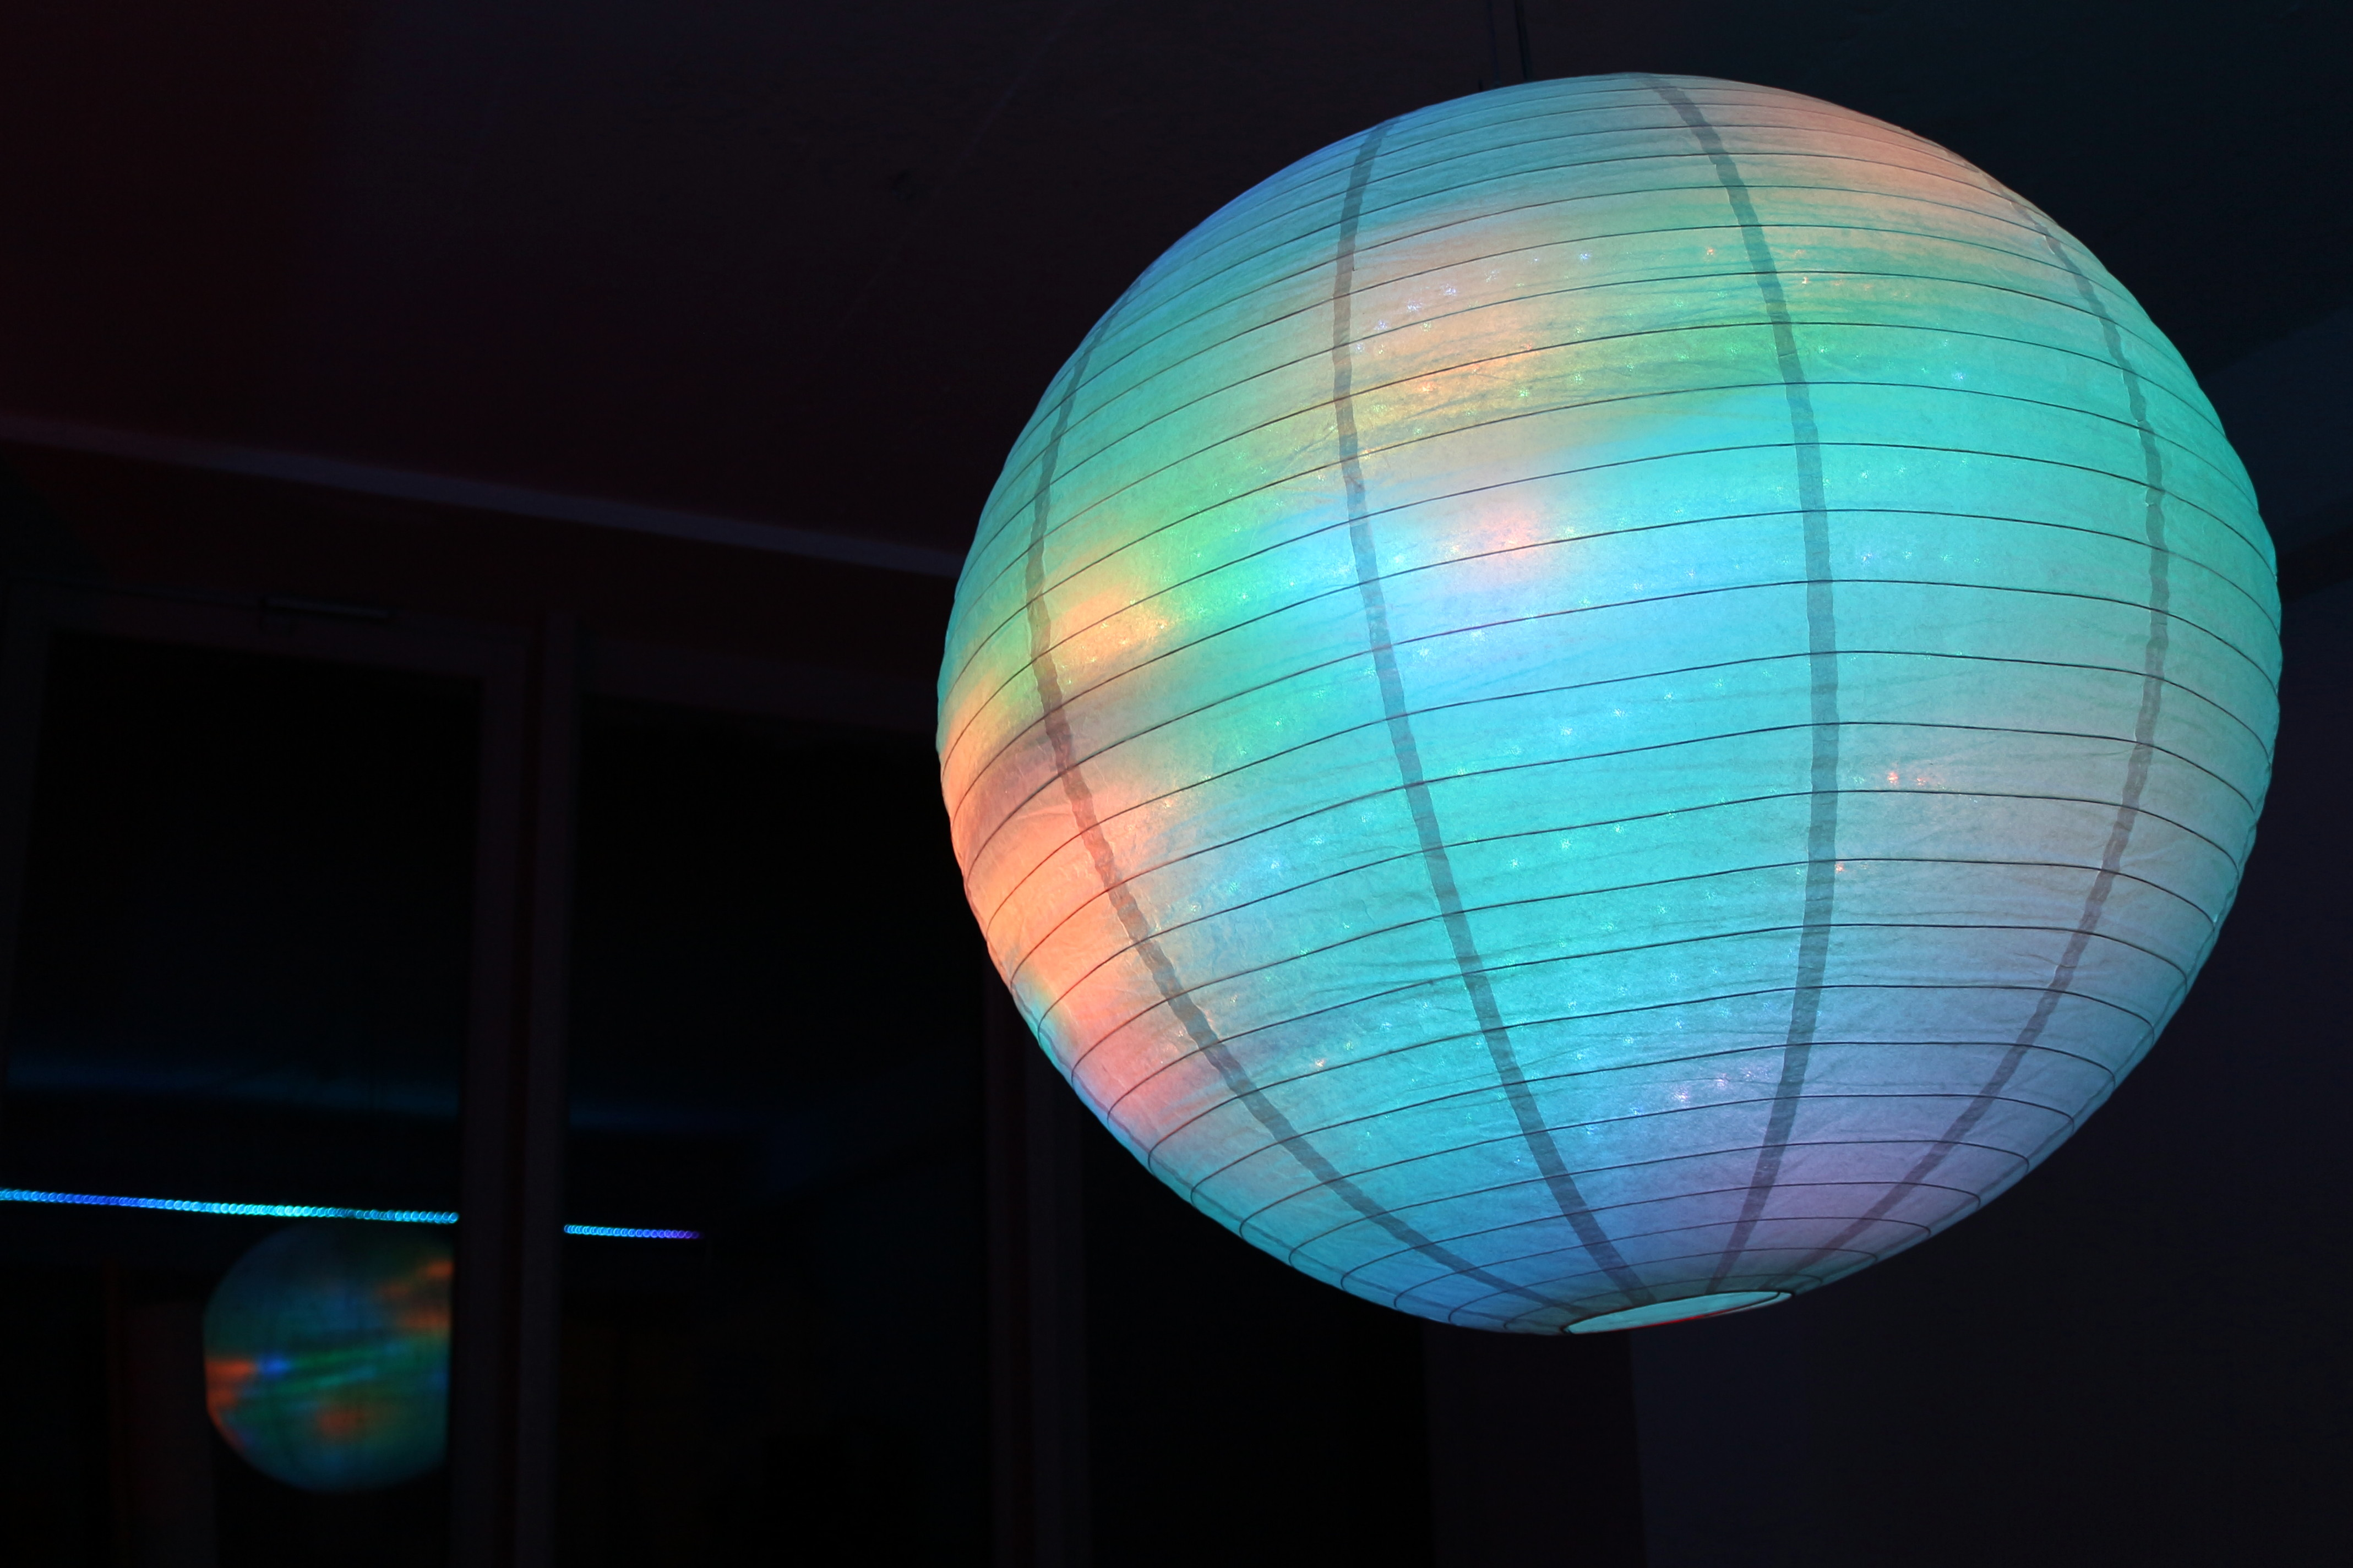
\includegraphics[height=0.7\textheight]{img/leds3.jpg}}
	\end{figure}
\end{frame}

\begin{frame}
	\frametitle{Einfache Formeln => hübsche Fraktale}
  	\begin{figure}
	    \only<1>{
	    	    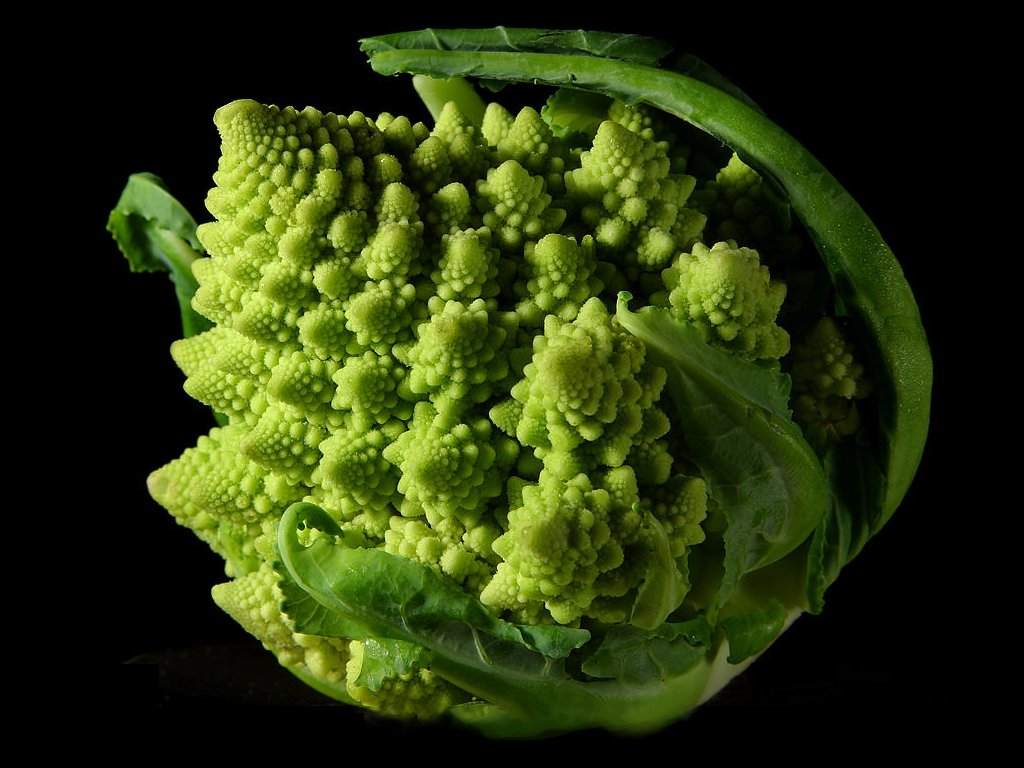
\includegraphics[height=0.7\textheight]{img/Fractal_Broccoli.jpg}
		    \tiny\license{https://upload.wikimedia.org/wikipedia/commons/4/4f/Fractal\_Broccoli.jpg}
	    }
	    \only<2>{
		    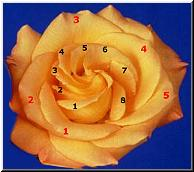
\includegraphics[height=0.5\textheight]{img/flower-petals-fibonacci.jpg}
		    \tiny\license{https://www.goldennumber.net/wp-content/uploads/2012/05/flower-petals-fibonacci.jpg}
	    }
	    \only<3>{
	    	    
\includegraphics[height=0.7\textheight]{img/snowflake.jpg}
		    \tiny\license{http://softology.com.au/gallery/gallery.htm}
	    }
	    \only<4>{
	    	    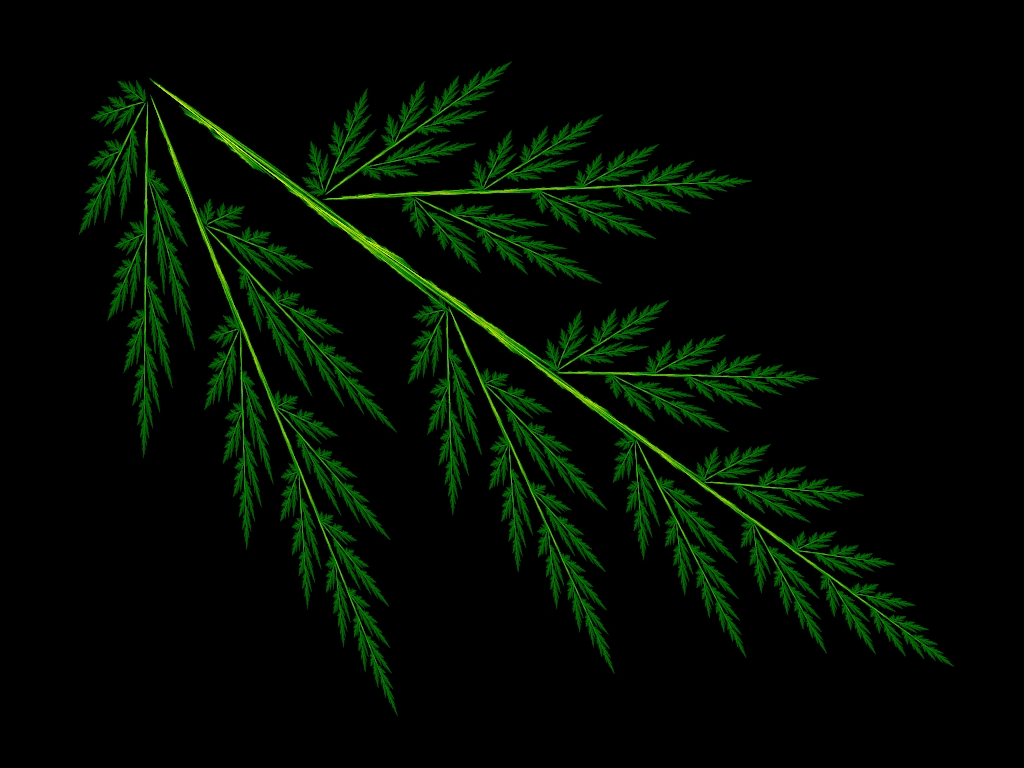
\includegraphics[height=0.7\textheight]{img/leaf.jpg}
		    \tiny\license{http://softology.com.au/gallery/gallery.htm}
	    }
	\end{figure}
\end{frame}

\begin{frame}
	\frametitle{Zelluläre Automaten}
  	\begin{figure}
	    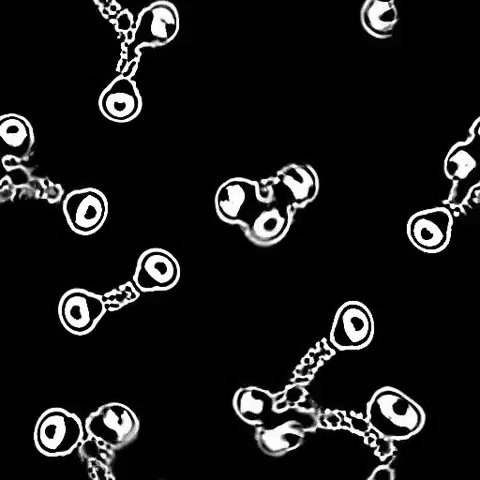
\includegraphics[height=0.7\textheight]{img/SmoothLiveL.jpg}
	    \tiny\license{https://www.youtube.com/watch?v=KJe9H6qS82I}
	\end{figure}
\end{frame}

\begin{frame}
	\frametitle{Neuronale Netze}
  	\begin{figure}
	    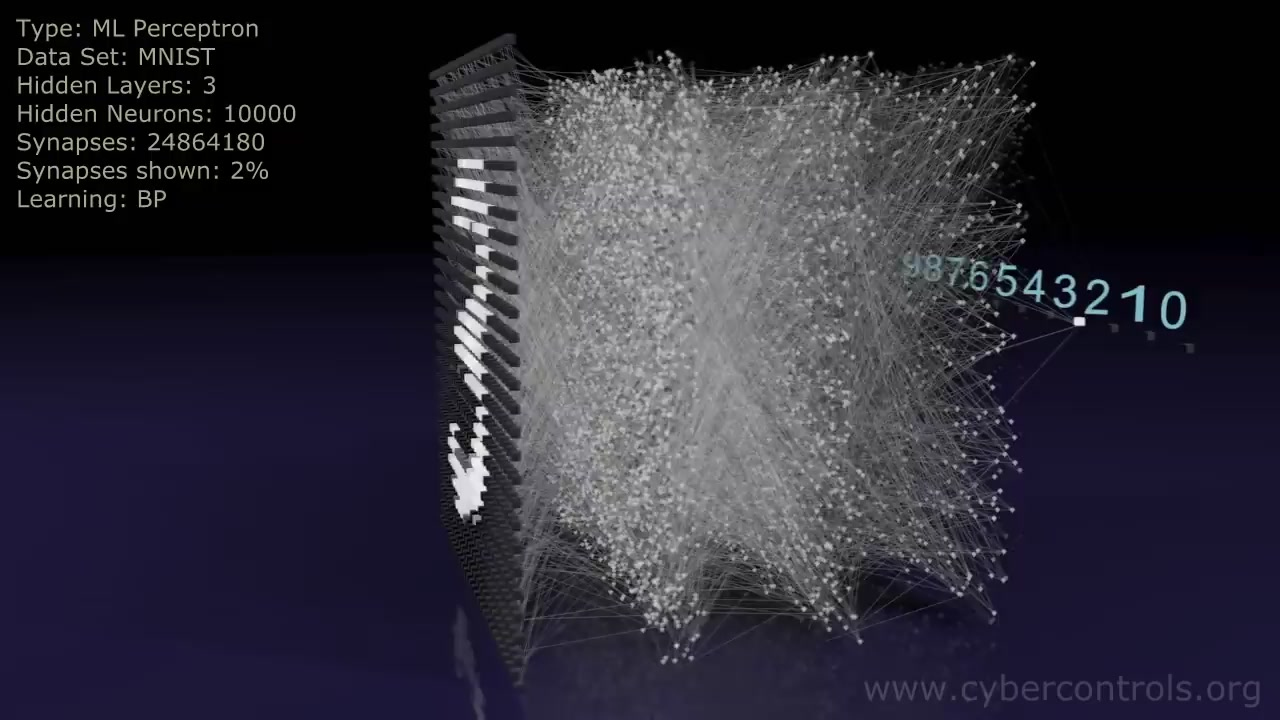
\includegraphics[height=0.7\textheight]{img/neuralNetwork.jpg}
	    \tiny\license{https://www.cybercontrols.org/}
	\end{figure}
\end{frame}

\begin{frame}
	\frametitle{Genetische Algorithmen}
  	\begin{figure}
	    \only<1>{
		    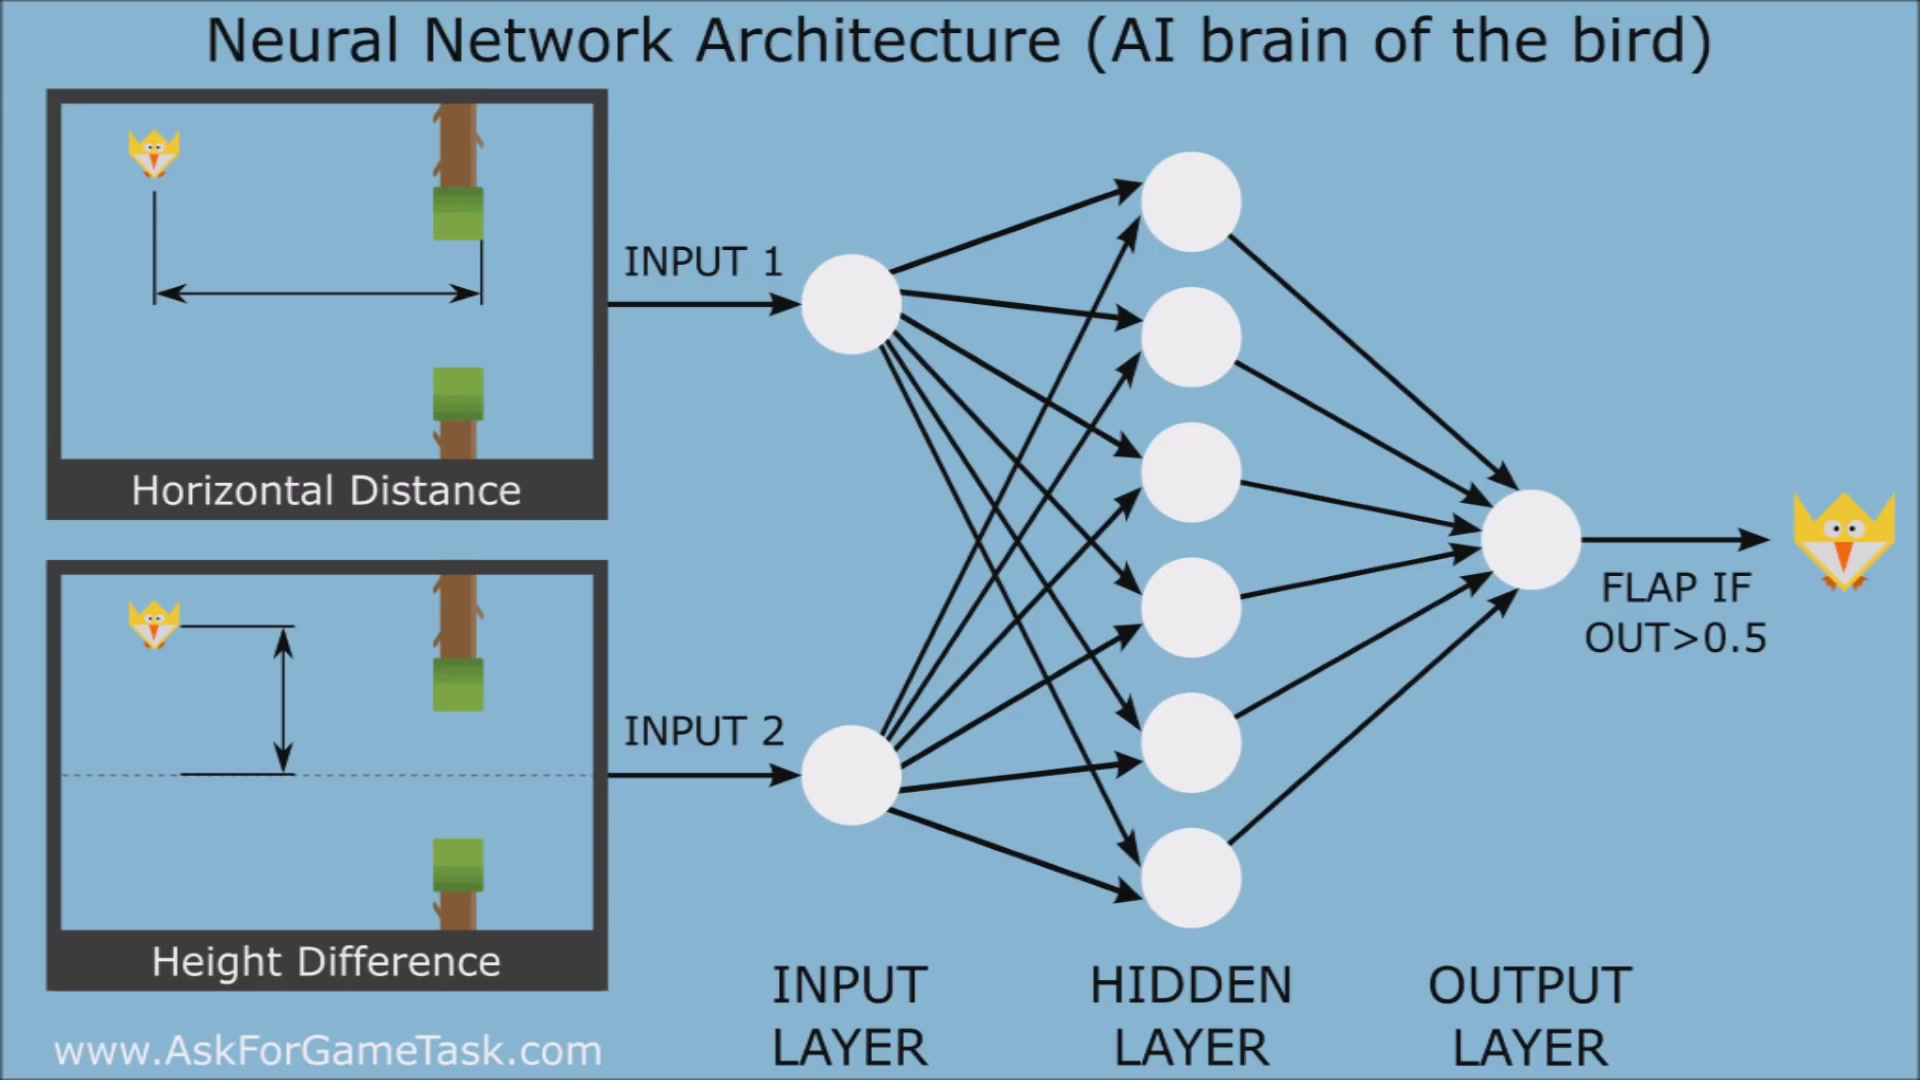
\includegraphics[height=0.7\textheight]{img/flappy1.jpg}
		    \tiny\license{https://www.askforgametask.com/}
	    }
	    \only<2>{
		    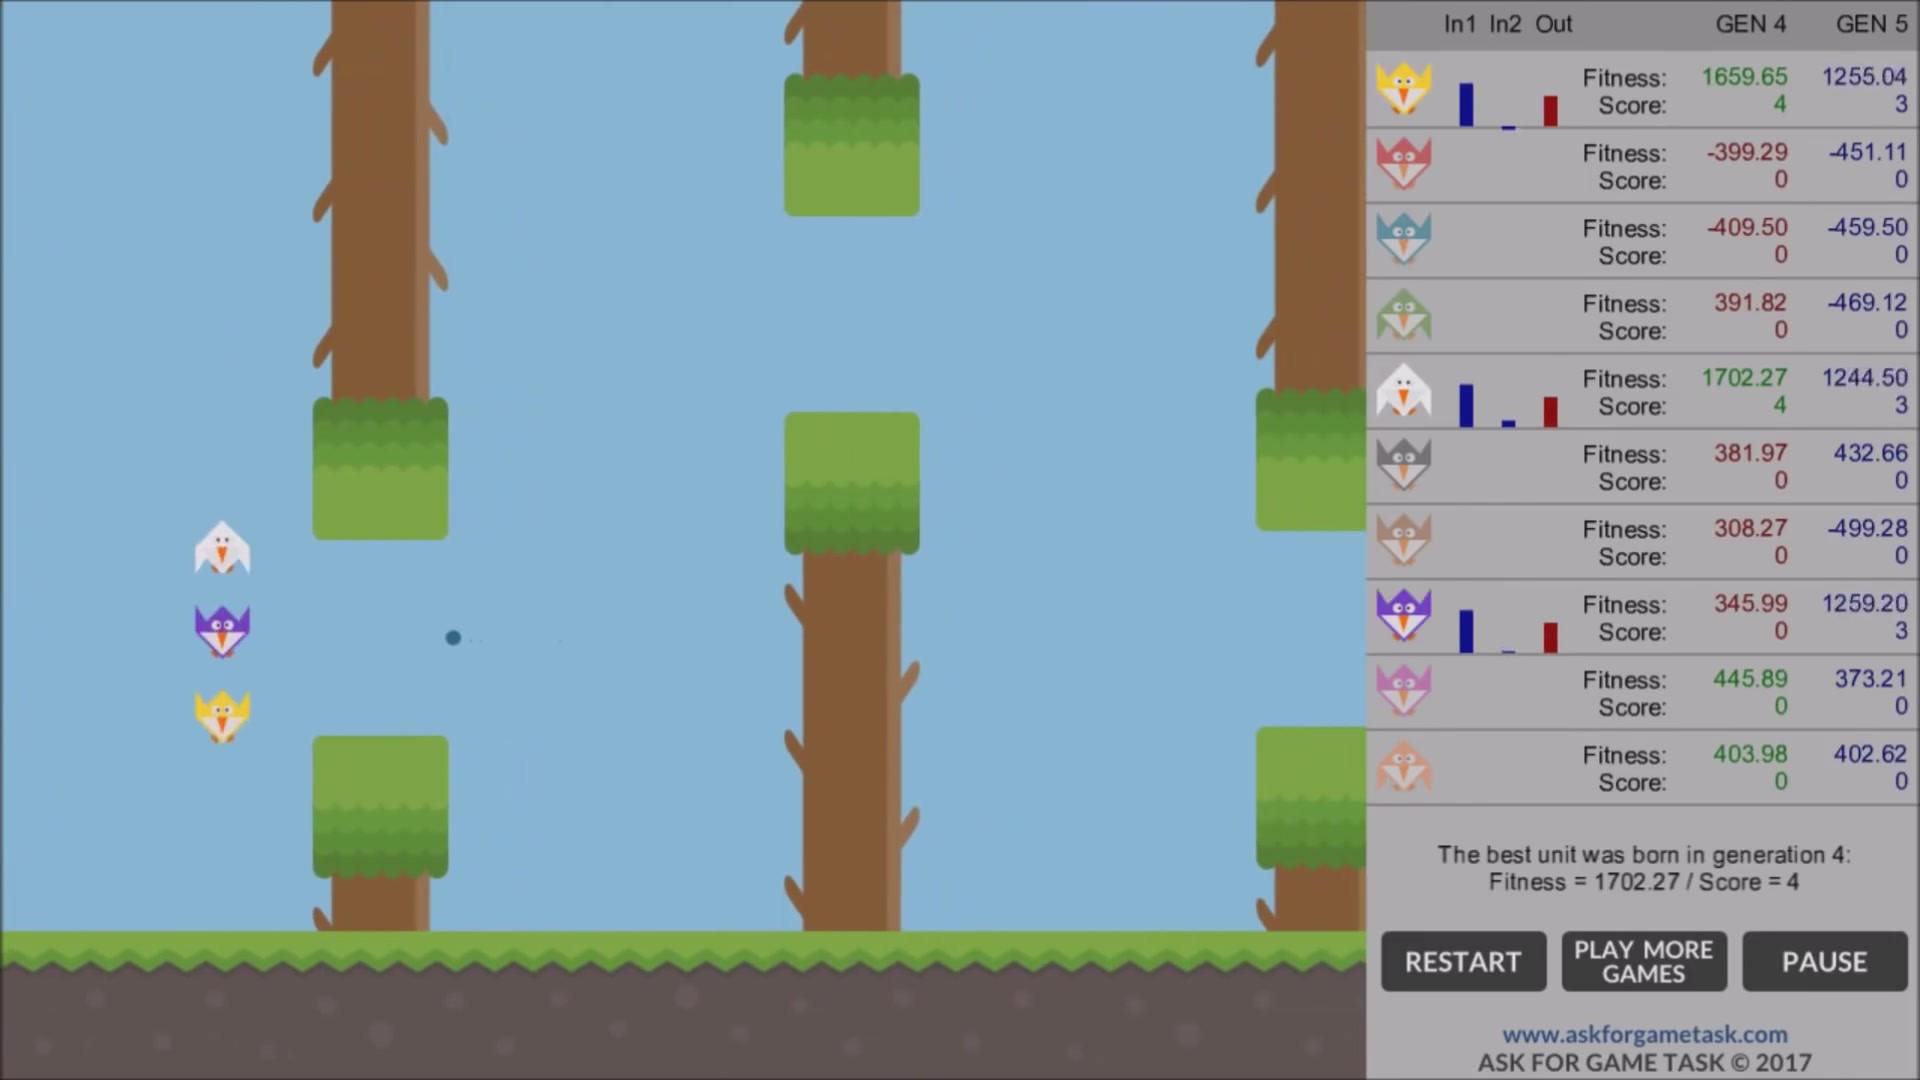
\includegraphics[height=0.7\textheight]{img/flappy2.jpg}
		    \tiny\license{https://www.askforgametask.com/}
	    }
	\end{figure}
\end{frame}


%%% -> Rob -> %%%


\begin{frame}
	\frametitle{Kolaborative Werkzeuge}
	Wikis
  	\begin{figure}
	    \only<1>{
		    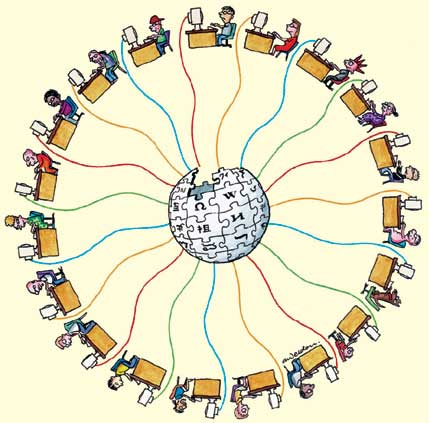
\includegraphics[height=0.7\textheight]{img/wiki_web_pupils.jpg}
		    \tiny\license{http://iwcmediaecology.pbworks.com/w/page/8480858/Wikis}
	    }
	\end{figure}
\end{frame}

\begin{frame}
	\frametitle{Kolaborative Werkzeuge}
	Pads (etherpad, piratenpad, hackmd, ..)
  	\begin{figure}
	    \only<1>{
		    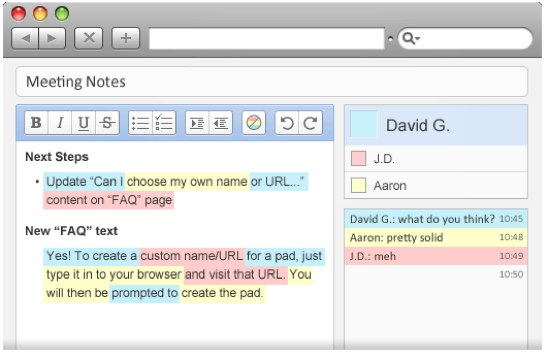
\includegraphics[height=0.7\textheight]{img/etherpad.jpg}
		    \tiny\license{https://techcrunch.com/2009/07/23/etherpad-gets-a-makeover-and-becomes-even-more-of-a-threat-to-google-docs/}
	    }
	    \only<2>{
		    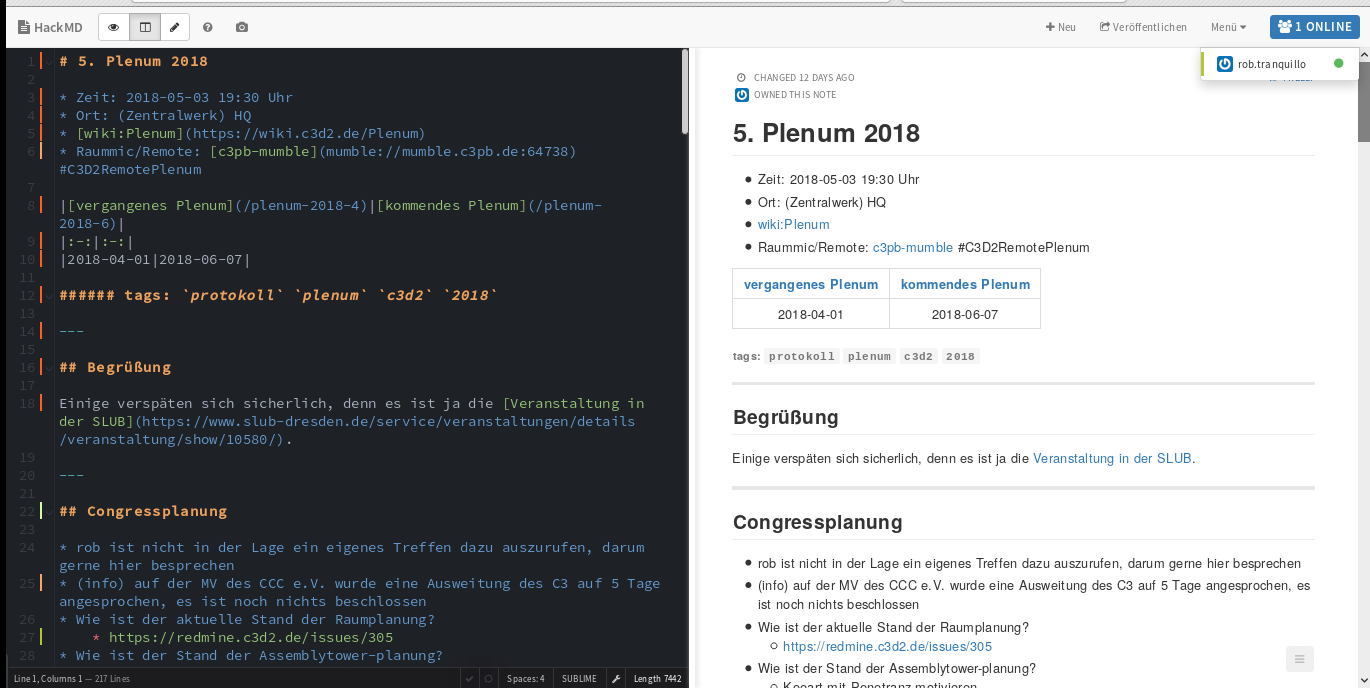
\includegraphics[height=0.7\textheight]{img/hackmd_c3d2.png}
		    \tiny\license{https://hackmd.c3d2.de}
	    }
	    \only<3>{
		    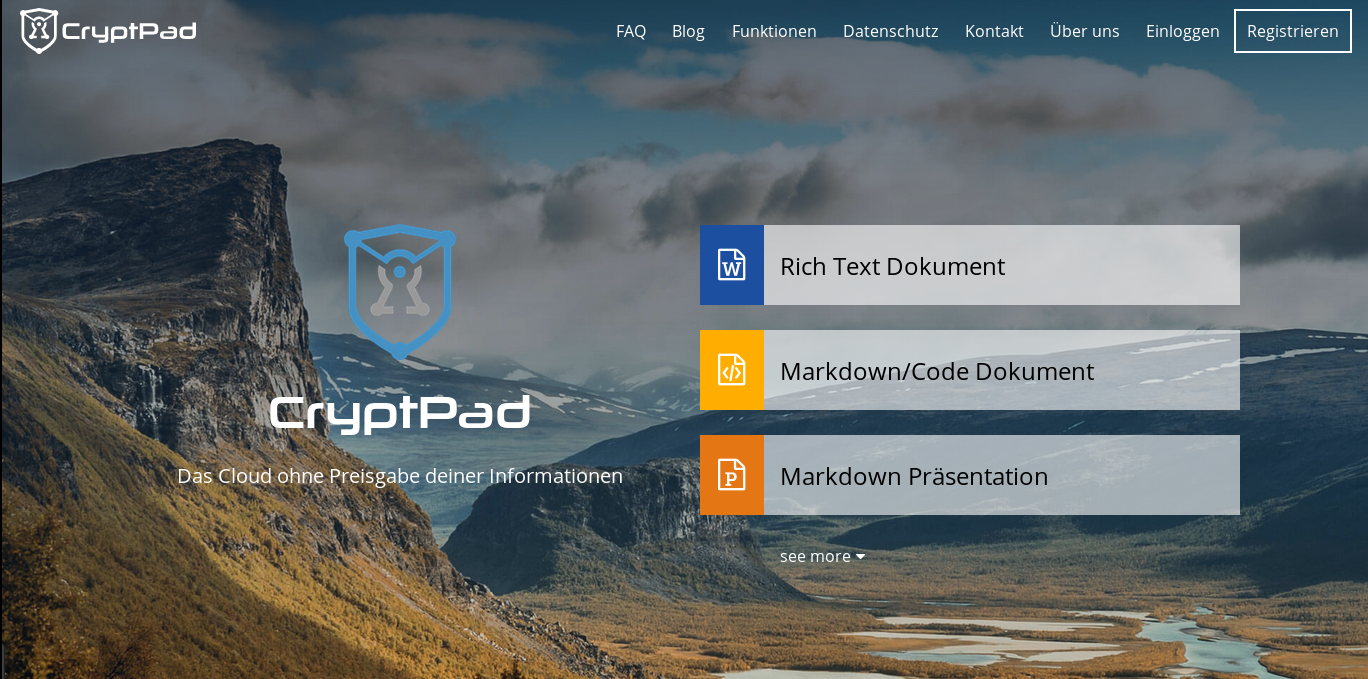
\includegraphics[height=0.7\textheight]{img/cryptpad.png}
		    \tiny\license{https://cryptpad.fr/}
	    }
	\end{figure}
\end{frame}

\begin{frame}
	\frametitle{Kolaborative Werkzeuge}
	Private Clouds
  	\begin{figure}
	    \only<1>{
		    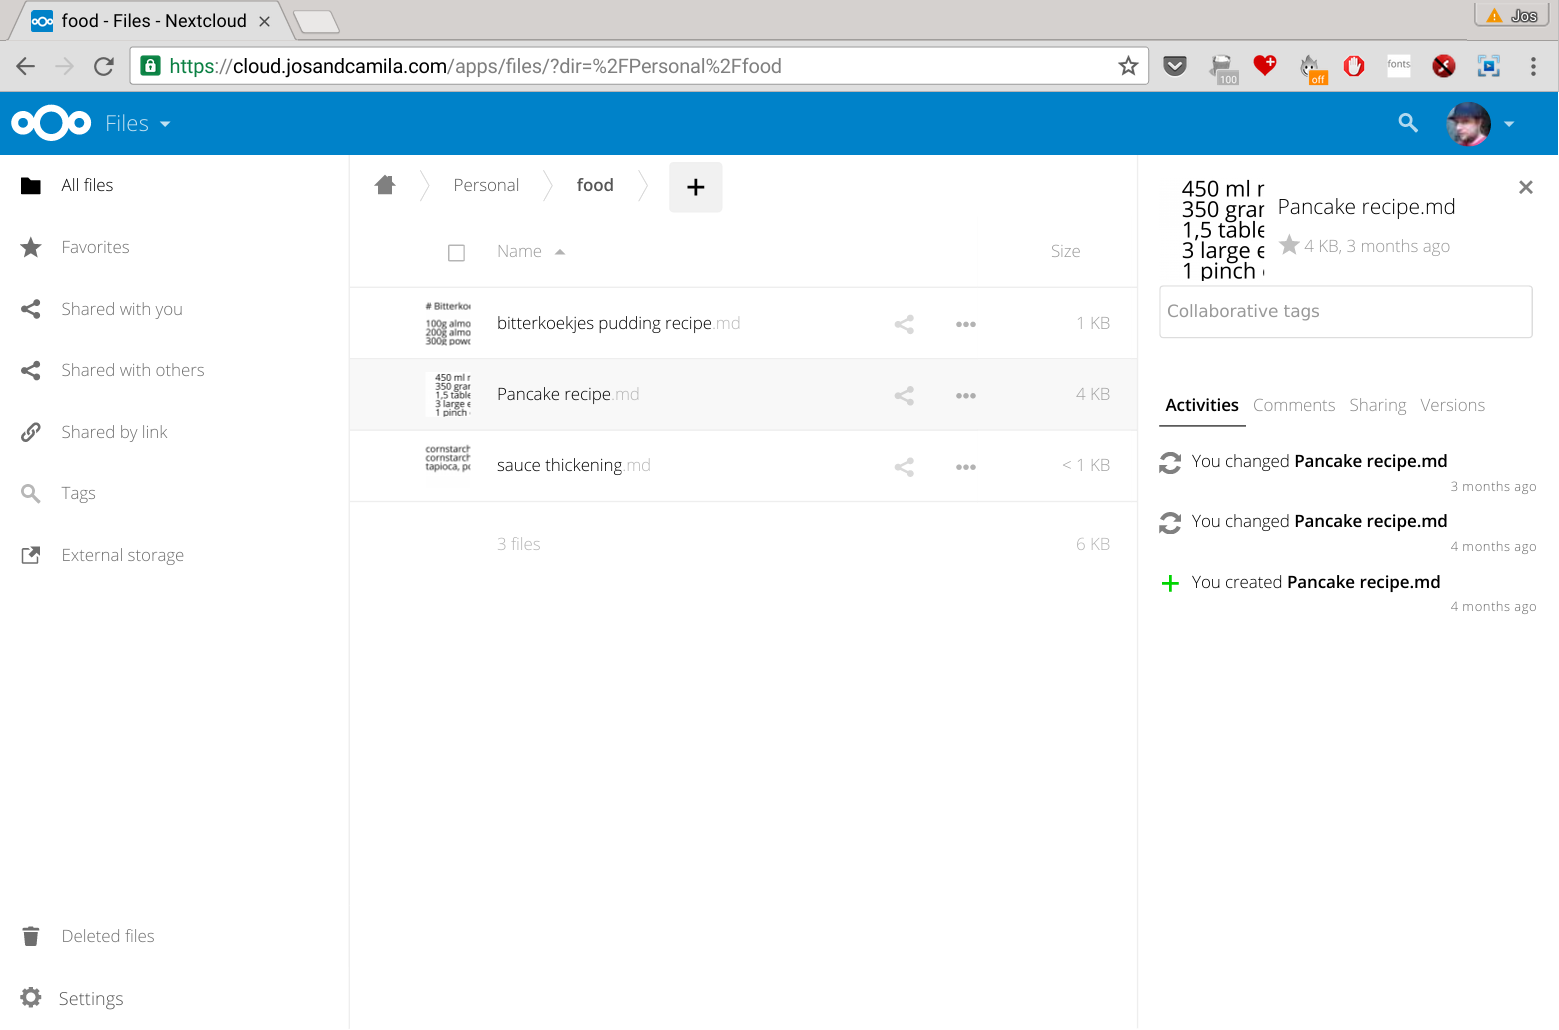
\includegraphics[height=0.7\textheight]{img/nextcloud.png}
		    \tiny\license{nextcloud.com}
	    }
	\end{figure}
\end{frame}

\begin{frame}
	\frametitle{Kolaborative Werkzeuge}
	Meinungsfindung
  	\begin{figure}
	    \only<1>{
		    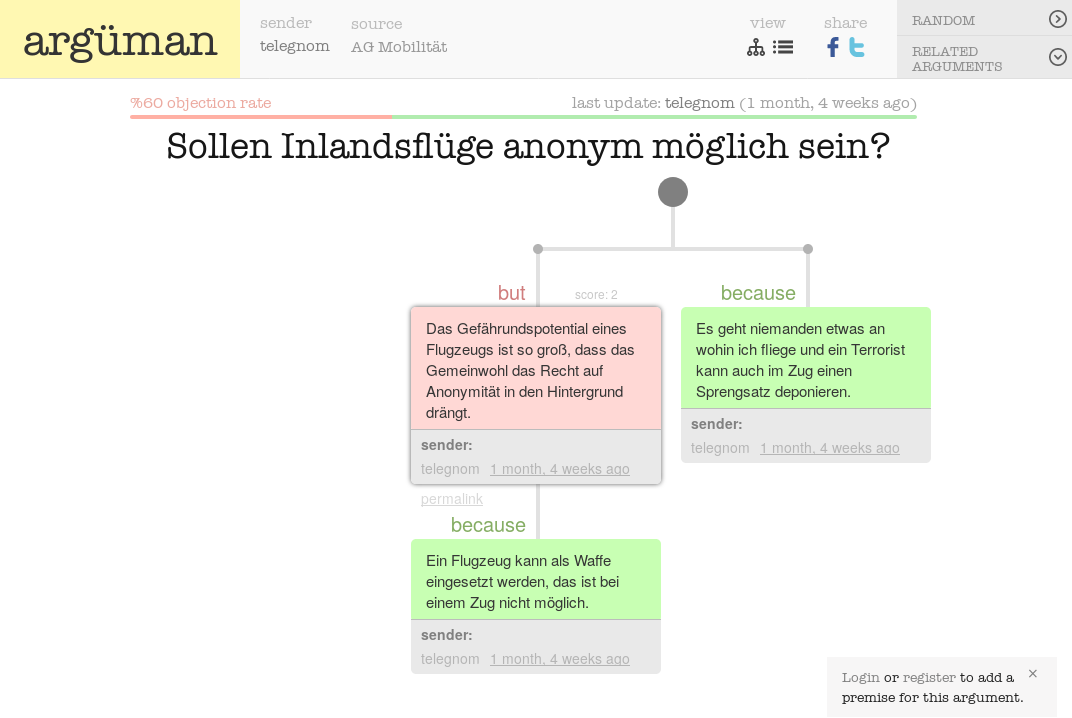
\includegraphics[height=0.7\textheight]{img/arguman.png}
		    \tiny\license{https://http://arguman.org}
	    }
	\end{figure}
\end{frame}


\section{Zukunft}
  \subsection{}
  
\begin{frame}
	\frametitle{Zukunft der Wirtschaft}
	\begin{itemize}
		\item<1-> Digitalisierung / Automatisierung
		\item<2-> Überwachung -> Daten!
		\item<3-> Daten -> Neuronale Netze
		\item<4-> DATEN!!!
	\end{itemize}
\end{frame}

\begin{frame}
	\frametitle{Ein Blick darüber hinaus..}
	\begin{itemize}
		\item<1-> Wissen und Vernetzung
		\item<2-> Technik Demokratisierung
		\item<3-> Freie Infrastrukturen
	\end{itemize}
\end{frame}


\begin{frame}
	\frametitle{Schlussworte}
	\begin{itemize}
		\item<1-> Zukunft?
		\item<2-> Lernen, Lehren, Lernen, Lehren
	\end{itemize}
\end{frame}

\section{Ende}
	\subsection{}

\begin{frame}
	\frametitle{Danksagung}
	\begin{center}
		\textbf{Ein Dank geht an:}
		\begin{itemize}
			\item<1-> die Fakultät für die Einladung
			\item<2-> an euch für das Interesse
			\item<3-> Autoren freier Software und Inhalte,\\ dank denen diese Präsentation möglich war  :-)
		\end{itemize}
	\end{center}
\end{frame}
  
\begin{frame}
	\frametitle{Ende}
	\begin{center}
		\textbf{Kontakt: schule@c3d2.de} \\
		\textbf{Fragen?} 
	\end{center}
	\begin{itemize}
		\item<1-> https://c3d2.de
		\item<2-> https://c3d2.de/schule.html
		\item<4-> https://lists.c3d2.de
	\end{itemize}
\end{frame}

\begin{frame}
	\begin{center}
    	
\includegraphics[height=0.5\textheight]{img//cms-text.png}
    \end{center}
\end{frame}

\end{document}
